\documentclass[12pt,a4paper,twoside]{article}
\usepackage{graphicx,xcolor,textpos}
\usepackage{helvet}
\usepackage[english]{babel}
\usepackage[normalem]{ulem}
\usepackage{amsmath}
\usepackage{amsthm}
\usepackage{thmtools,thm-restate}
\usepackage{bbm}
\usepackage{amssymb}
\usepackage{hyperref}
\usepackage{relsize}
\usepackage[margin=0.7in]{geometry}
\usepackage{physics}
\usepackage{enumitem}
\usepackage{mathtools}
\usepackage{changepage}
\usepackage{caption}
\usepackage{subcaption}
\usepackage{verbatim}
\usepackage{url}
\usepackage{standalone}
\usepackage{tikz}
\usetikzlibrary{calc,patterns,angles,quotes}

\newcommand{\stkout}[1]{\ifmmode\text{\sout{\ensuremath{#1}}}\else\sout{#1}\fi}
\renewcommand{\d}{\text{d}}
\renewcommand{\O}{\mathcal{O}}
\newcommand{\e}{\mathlarger{e}}
\newcommand{\defeq}{\vcentcolon=}

\let\originalleft\left
\let\originalright\right
\renewcommand{\left}{\mathopen{}\mathclose\bgroup\originalleft}
\renewcommand{\right}{\aftergroup\egroup\originalright}
\title{A $H^2(G,\TT)\oplus H^3(G,\TT)$-valued index for SPT states with translation symmetry in two dimensional quantum spin systems}
\author{Tijl Jappens}
\date{\today}

\newcommand{\UU}{\mathcal U}
\newcommand{\KK}{\mathcal K}
\newcommand{\BB}{\mathcal B}
\newcommand{\PP}{\mathcal P}
\newcommand{\HH}{\mathcal H}
\newcommand{\ZZ}{\mathbb Z}
\newcommand{\CC}{\mathbb C}
\newcommand{\TT}{\mathbb T}
\renewcommand{\AA}{\mathcal A}
\newcommand{\LL}{\mathcal L}
\newcommand{\RR}{\mathbb R}
\newcommand{\NN}{\mathbb{N}}
\newcommand{\id}{\mathbbm{1}}

\newcommand{\Ad}[1]{\textrm{Ad}\left(#1\right)}
\newcommand{\Aut}[1]{\textrm{Aut}\left(#1\right)}
\newcommand{\QAut}[1]{\textrm{QAut}\left(#1\right)}

\newcommand{\qe}{\underset{\text{q.e.}}{\sim}}
\newcommand{\ue}{\underset{\text{u.e.}}{\sim}}

\newcommand{\Mod}[1]{\mathrm{mod} #1}

\theoremstyle{definition}
\newtheorem{theorem}{Theorem}[section]
\newtheorem{definition}[theorem]{Definition}
\newtheorem{lemma}[theorem]{Lemma}
\newtheorem{remark}[theorem]{Remark}
\newtheorem{assumption}[theorem]{Assumption}
\newtheorem{conjecture}[theorem]{Conjecture}

\numberwithin{equation}{section}
\begin{document}
\maketitle	
\begin{abstract}
	content...
\end{abstract}
\section{Introduction}
The notion of symmetry protected topological phases of matter was introduced by Gu and Wen \cite{Chen_2013}. One possible setup in which one can define spt phases is in quantum spin systems (defined in the next section). To define spt phases one needs to fix a group $G$ with an on site group action $\beta_g$ (see the next section for more information). Then one needs to impose a restriction on the space of states. One possible\footnote{There are other definitions possible like for instance the concept of invertible G-invariant states.} way to do this is to say that a state $\omega_1$ is now an spt state for a symmetry group $G$ if there exists a $G$-invariant, bounded interaction $\Phi_1$ (defined in section 1 in \cite{ogata2021h3gmathbb}) such that
\begin{enumerate}
	\item $\omega_1$ is the unique gapped groundstate of $\Phi_1$.
	\item there is a path\footnote{for the precise definitions of what these paths of interactions must satisfy we refer to section 1 in \cite{ogata2021h3gmathbb}} of interactions with a uniform lower bound on the gap (but not necessarily $G$-invariant) that connects $\Phi_1$ to a trivial interaction (one whose unique gapped groundstate is a product state).
\end{enumerate}
One then defines an equivalence class on these spt states by saying that $\omega_1$ (a unique gapped groundstate of $\Phi_1$) is equivalent to $\omega_2$ (a unique gapped groundstate of $\Phi_2$) if there exists a $G$-invariant path of interactions (with a uniform lower bound on the gap) connecting $\Phi_1$ and $\Phi_2$. The space of equivalence classes of spt states is then called the spt classification. In one spacial dimension it was shown by Yoshiko Ogata \cite{ogata2019classification} that any state satisfying the split property (this includes both gapped groundstates of local Hamiltonians and invertible states) carries an $H^2(G,\TT)$-valued\footnote{By $H^n(G,\TT)$ we mean the n-th Borel group cohomology of $G$ with coefficients in the torus $\TT$. This is equivalent to the singular cohomology with coefficients in $\TT$ of the classifying space $BG$ of $G$.} index and that this index is invariant under this equivalence class. Later on Anton Kapustin, Bowen Yang and Nikita Sopenko \cite{kapustin2021classification} then showed that this classification problem is complete (the index is injective) if one looks at invertible states under stable equivalence. In two spatial dimensions more recently Yoshiko Ogata \cite{ogata2021h3gmathbb} proved there is an $H^3(G,\TT)$-valued index this time belonging to the classification problem as presented here that is protected under this equivalence class.
\\\\
The goal of this paper is to look at the 2d case with the equivalence class as presented here but with one notable difference. We will only consider states and interactions that have a translation symmetry in one direction. There is a long standing conjecture about the spt classification of such states. See for instance \cite{xiong2019classification} section 3.1.5.1 where they present this conjecture in a very general way. It goes as follows:
\begin{conjecture}\label{conj}
	Let $g$ be the inclusion map from the space of 2d translation invariant spt states to the more general set of 2d spt states. Let $f$ be the map that takes a 1d spt state and outputs a translation invariant 2d spt state by taking the tensor product in the direction of the translation symmetry. The sequence
	\begin{equation}
		0\rightarrow\{\text{1d spt states}\}\stackrel{f}{\rightarrow}\{\text{2d translation invariant spt states}\}\stackrel{g}{\rightarrow}\{\text{2d spt states}\}\rightarrow 0
	\end{equation}
	induces a sequence on the equivalence classes. By this we mean that the class of $f(\phi)$ only depends on the class of $\phi$ and similarly for $g$. Moreover this induced sequence is exact and split.
\end{conjecture}
Clearly this implies that
\begin{equation}
	\{\text{2d translation invariant spt classification}\}\simeq \{\text{1d spt classification}\}\oplus \{\text{2d spt classification}\}.
\end{equation}
Since a 1d spt state carries an $H^2(G,\TT)$ valued index and a 2d spt state carries an $H^3(G,\TT)$ valued index this means that 2d spt states with a translation symmetry should carry an $H^2(G,\TT)\oplus H^3(G,\TT)$ valued index.\\\\
The main goal of this paper is now to find an $H^2(G,\TT)$ valued index (which we will denote by $\textrm{Index}$) on the space of translation invariant spt states that is consistent with the conjecture. By being consistent with the conjecture it is meant that if $\textrm{Index}_1$ is the one dimensional spt index from \cite{ogata2019classification} that then $\textrm{Index}(f(\omega))=\textrm{Index}_1(\omega)$ for any 1d spt $\omega$.\\\\
We will also look at the case where there is a second translation symmetry (so the system is translation invariant in both $x$ and $y$ directions). For this there is also a conjecture:
\begin{conjecture}\label{conj2}
	Let $g$ be the inclusion map from the space of 2d spt states that are translation invariant in both $x$ and $y$ directions to the more general set of 2d spt states with translation invariance in the $x$ direction only. Let $f$ be the map that takes a 1d translation invariant spt state and outputs a 2d spt state that is translation invariant in both $x$ and $y$ directions by taking the tensor product in the $y$ direction. The sequence
	\begin{equation}
		0\rightarrow\left\{\begin{matrix}\text{1d translation invariant}\\ \text{spt states}\end{matrix}\right\}\stackrel{f}{\rightarrow}\left\{\begin{matrix}\text{2d spt states with two}\\ \text{translation symmetries}\end{matrix}\right\}\stackrel{g}{\rightarrow}\left\{\begin{matrix}\text{2d spt states translation}\\ \text{invariant in $x$ direction}\end{matrix}\right\}\rightarrow 0
	\end{equation}
	induces a sequence on the equivalence classes. By this we mean that the class of $f(\phi)$ only depends on the class of $\phi$ and similarly for $g$. Moreover this induced sequence is exact and split.
\end{conjecture}
1d spt states are known to carry an $H^2(G,\TT)\oplus H^1(G,\TT)$ valued index (see appendix \ref{sec:OneDimensionalIndices}). From this and the conjecture, we expect there to be an
\begin{equation}\label{eq:2TranslationsIntroduction}
	H^3(G,\TT)\oplus H^2(G,\TT)\oplus H^2(G,\TT)\oplus H^1(G,\TT)
\end{equation}
valued index. The first part of the index is just $\textrm{Index}_{2d}$. The following two parts can be related to the case of one translation symmetry as follows. Let $\mu$ be the automorphism that rotates the $C^*$ algebra by 90° and let $\textrm{Index}(\omega)$ be the index as constructed before (this is the second part of \ref{eq:2TranslationsIntroduction}). The third part of the index is now given by $\textrm{Index}(\omega\circ\mu)$ (the state rotated by 90°). The last part of the index requires a different construction altogether and can be thought of as being the charge in the Brillouin zone.\\\\
The layout of this paper will be as follows: First in section \ref{sec:Setup} we explain the setup, and define the concept of locally generated automorphisms. Then in section \ref{sec:Results_1} we state the two results for states that are short range entangled (this is condition is strictly weaker then the one we talked about before). Then in section \ref{sec:Results_2}, we state the first result using a the weaker assumption \ref{assumption} and the second result using the weaker assumption \ref{assumption:2Translations}. It is using these weaker assumptions that we will prove the statements. Section \ref{sec:ProofFirstStatement} will then provide a proof of the first statement whereas section \ref{sec:TwoDirectionTraslationInvariance} will provide a proof of the second statement.
\section{Setup and definitions}\label{sec:Setup}
In what follows let $\AA$ be a quasi-local $C^*$ algebra defined on a two dimensional square lattice (see eg. \cite{ogata2021h3gmathbb} section 1). Let $G$ be a group and let $U_i\in\hom(G,\AA_i)$ (for $i\in\ZZ^2$) be the on site group action. Take $\beta^\Gamma\in\hom(G,\Aut{\AA_\Gamma})$ (for any $\Gamma\subset\ZZ^2$) be such that
\begin{equation}
	\beta^\Gamma_g(A)=\Ad{\otimes_{i\in I} U_i(g)}(A)
\end{equation}
for any $g\in G$, $I\subset\Gamma$ finite and $A\in\AA_I$. Let
\begin{align}
	L&\defeq \left\{(x,y)\in\ZZ^2\left|x<0\right.\right\},&R&\defeq \left\{(x,y)\in\ZZ^2\left|x\geq 0\right.\right\}\\
	U&\defeq \left\{(x,y)\in\ZZ^2\left|y\geq 0\right.\right\},&D&\defeq \left\{(x,y)\in\ZZ^2\left|y<0\right.\right\}
\end{align}
be the left, right, upper and lower half planes respectively and let
\begin{equation}
	C_\theta\defeq \left\{(x,y)\in\ZZ^2\left|\tan(\theta)\leq\abs{\frac{y}{x}}\right.\right\}
\end{equation}
be the horizontal cone (the green area on figure \ref{fig:SetupWithQAutomorphism}). We will use $\tau$ to denote the automorphism that moves every element of $\AA$ one site upward. Of course this is only an automorphism if the $C^*$ algebra is translation invariant in the vertical direction which we will assume. In the case where we have translation invariance in both directions we will obviously require the $C^*$ algebra to be translation invariant in both directions. In this case we will denote the translation automorphism that translates every element to the right by $\nu$. In this setup we will also assume that the group action acts in a translation invariant way ($\tau\circ\beta_g^\Gamma=\beta_g^{\tau(\Gamma)}\circ\tau$). We will sometimes also denote $\tau(Z)$ for some $Z\subset\ZZ^2$ to also denote the set that has been moved up by one site without using a different symbol for it. In what follows we will sometimes need to widen our cone vertically by one site. For this purpose we define $W$ such that
\begin{equation}
	W(C_\theta)\defeq C_\theta\cup\tau(C_\theta)\cup\tau^{-1}(C_\theta).
\end{equation}
In the later parts of the paper we will also need the automorphism that rotates every element of the $C^*$ algebra by $90^\circ$ (clockwise) which we will call $\mu$.\footnote{We will not discuss rotation invariant states in this paper. The $\mu$ is only defined to make certain constructions work.}
\subsection{Interactions and locally generated automorphisms}
In what follows let $\mathfrak{G}_{\ZZ^2}$ be the set of finite subsets of $\ZZ^2$. An interaction $\Phi$ is a map
\begin{equation}
	\Phi: \mathfrak{G}_{\ZZ^2}\rightarrow \AA_{\text{loc}}: I \mapsto \Phi(I)
\end{equation}
where $\Phi(I)\in\AA_I$. We will sometimes require a norm on the space of interactions that indicates how local an interaction acts.Take $F:\NN\rightarrow \RR^+$ any monotonically decreasing positive function then we define an $F$-norm on the space of interactions by:
\begin{equation}
	\norm{\Phi}_F\defeq \sup_{x,y\in\ZZ^2}\frac{1}{F(\abs{x-y})}\sum_{Z\in\mathfrak{G}_{\ZZ^2},Z\ni x,y}\norm{\Phi(Z)}.
\end{equation}
Following \cite{ogata2021h3gmathbb} we will fix a specific family of monotonically decreasing positive functions by saying that for any $0<\phi<1$ we define
\begin{equation}
	F_\phi:r\mapsto \frac{\exp(-r^\phi)}{(1+r)^4}.
\end{equation}
We will sometimes use the restriction of an interaction. For some $\Gamma\subset\ZZ^2$ we define $\Phi_\Gamma$ by
\begin{equation}
	\Phi_\Gamma:\mathfrak{G}_{\ZZ^2}\rightarrow \AA_{\text{loc}}:I\mapsto\left\{\begin{matrix}
		\Phi(I)&\text{if }I\subset\Gamma\\0&\text{otherwise}.
	\end{matrix}\right.
\end{equation}
One of the properties of $F$-local interactions is that they can be used to generate automorphisms. Let
\begin{equation}
	\Phi:\mathfrak{G}_{\ZZ^2}\times [0,1]\rightarrow \AA_{\text{loc}}:(I,t)\mapsto \Phi(I,t)
\end{equation}
be a one parameter family of interactions such that the $F$-norm is uniformly bounded ($\sup_{t\in[0,1]}\norm{\Phi(\cdot,t)}_F<\infty$). We will call the set of one parameter families of interactions that satisfy this property $\BB_{F}([0,1])$. For any $\Phi\in\BB_{F_\phi}([0,1])$, we define the locally generated automorphism $\gamma^{\Phi}_{s;t}$ such that for any $A\in\AA$, $\gamma^{\Phi}_{s;t}(A)$ is given as the solution to the differential equation
\begin{equation}
	\frac{\d}{\d t}\gamma^{\Phi}_{s;t}(A)=-i\sum_{I\in\mathfrak{G}_{\ZZ^2}}\gamma^{\Phi}_{s;t}([\Phi(I,t),A])
\end{equation}
with initial condition $\gamma^{\Phi}_{s;s}(A)=A$. Sometimes we will say that an interaction is $G$-invariant. By this we simply mean that $\beta_g(\Phi(I))=\Phi(I)$ (for all $I\in\mathfrak{G}_{\ZZ^2}$). Similarly if we say an interaction is translation invariant we mean that $\tau(\Phi(I))=\Phi(\tau(I))$ (for all $I\in\mathfrak{G}_{\ZZ^2}$). It should be clear that if an interaction is $G$-invariant (translation invariant) that then the lga it generates commutes with the group action (the translation automorphism) as well.
\section{Results}
We will present our claim starting from two different assumptions. The first assumption is related to short range entanglement whereas the second assumption is more technical but also more general (the first assumption will imply the second assumption).
\subsection{Statement of the results in therms of short range entanglement}\label{sec:Results_1}
We can use these locally generated automorphisms to define the concept of short range entanglement.
\begin{definition}
	Take $\omega\in\PP(\AA)$. We say that $\omega$ is a short range entangled state (in short an sre state) if and only if there exists a one parameter family of interactions $\Phi\in\BB_{F_\phi}([0,1])$ (for some $0<\phi<1$) such that $\omega\circ\gamma^{\Phi}_{0;1}$ is a product state. We then call $\gamma^{\Phi}_{0;1}$ a disentangler for $\omega$.
\end{definition}
We can now formulate our first result for the case where there is one translation symmetry.
\begin{theorem}
	There exists a map
	\begin{equation}
		\textrm{Index}:\{\omega\in\PP(\AA)|\omega\text{ is an sre state},\omega\circ\beta_g=\omega\text{ and }\omega\circ\tau=\omega\}\rightarrow H^2(G,\TT)
	\end{equation}
	that is well defined (doesn't depend on $\omega_0$ or the choice of disentangler). This map will be consistent with conjecture \ref{conj}. By this we mean that:
	\begin{enumerate}
		\item For any $G$ and translation invariant family of interactions $\Phi\in\BB_{F_{\phi}}([0,1])$ (for some $0<\phi<1$) we have that
		\begin{equation}
			\textrm{Index}(\omega)=\textrm{Index}(\omega\circ\gamma^{\Phi}_{0;1}).
		\end{equation}
		\item Take $\phi$ a one dimensional short ranged entangled $G$-invariant state then the (infinite) tensor product of this state in the vertical direction (see section \ref{sec:OneTranslationDirectionExample} definition \ref{def:InfiniteTensorProductState}), $\omega$ satisfies
		\begin{equation}
			\textrm{Index}_{1d}(\phi)=\textrm{Index}(\omega)
		\end{equation}
		where $\textrm{Index}_{1d}$ is defined in appendix \ref{sec:OneDimensionalIndices}.
	\end{enumerate}
\end{theorem}
\begin{proof}
	{\color{red}Todo}
\end{proof}
Now for the second result I would like to define an index on the space of $G$-invariant sre states that is translation invariant in both the horizontal and the vertical directions. In the introduction we already stated that the conjecture indicates that this is classified by $H^3(G,\TT)\oplus H^2(G,\TT)\oplus H^2(G,\TT)\oplus H^1(G,\TT)$. The first index is just the index when there are no translations. Clearly there are two other indices one can define already. Namely, take
\begin{align}
	\omega&\mapsto \textrm{Index}(\omega)&&\text{and}&\omega\mapsto \textrm{Index}(\omega\circ\mu)
\end{align}
where $\mu$ was the rotation automorphism. This will give the $H^2(G,\TT)\oplus H^2(G,\TT)$ part. The second result presented in this paper is that we can also define this $H^1(G,\TT)$\footnote{There is a result from group cohomology that $H^1(G,\TT)\cong\hom(G,\TT)$. We will use this identification freely.} index.
\begin{theorem}
	There exists a map
	\begin{equation}
		\textrm{Index}_{2\text{ trans}}:\left\{\omega\in\PP(\AA)\left| \begin{matrix}\omega\text{ is an sre state,}\\\omega\circ\beta_g=\omega,\:\omega\circ\tau=\omega\text{ and }\omega\circ\nu=\omega\end{matrix} \right.\right\}\rightarrow H^1(G,\TT)
	\end{equation}
	that is well defined (doesn't depend on $\omega_0$ or the choice of disentangler). This map will be consistent with conjecture \ref{conj2}. By this we mean that:
	\begin{enumerate}
		\item For any $G$ invariant family of interactions that is translation invariant in both directions $\Phi\in\BB_{F_\phi}([0,1])$ we have that
		\begin{equation}
			\textrm{Index}_{2\text{ trans}}(\omega)=\textrm{Index}_{2\text{ trans}}(\omega\circ\gamma^\Phi_{0;1}).
		\end{equation}
		\item Let $\phi$ be a one dimensional short ranged entangled $G$-invariant translation invariant state then the (infinite) tensor product of this state in the vertical direction satisfies
		\begin{equation}
			\textrm{Index}_{1d\text{ trans}}(\phi)=\text{Index}_{2\text{ trans}}(\omega)\footnote{$\textrm{Index}_{1d\text{ trans}}$ is defined in appendix \ref{sec:OneDimensionalIndices}.}.
		\end{equation}
		\item Let $\mu$ be the automorphism that rotates every element of the $C^*$ algebra by $90^\circ$ degrees then
		\begin{equation}
			\textrm{Index}_{\text{2 trans}}(\omega)=\textrm{Index}_{\text{2 trans}}(\omega\circ\mu).
		\end{equation}
	\end{enumerate}
\end{theorem}
\begin{proof}
	{\color{red}Todo...}
\end{proof}
\subsection{Statement of the result in therms of Q-automorphisms}\label{sec:Results_2}
\documentclass[preview=false]{standalone}
\begin{document}

\begin{figure}
	\centering
	\def\s{0.5}
	\resizebox{0.4\textwidth}{!}{%
		\begin{tikzpicture}
			\fill[fill=blue!30!white] (-4*\s,-4*\s) rectangle (4*\s,4*\s);
			\draw[draw=black,line width=0.5mm] (0,4*\s) -- (0,-4*\s);
			
			\node at (-2*\s,0) {$\alpha_L$};
			\node at (2*\s,0) {$\alpha_R$};
		\end{tikzpicture}}
	$\qquad$
	\def\s{0.4}
	\resizebox{0.32\textwidth}{!}{%
		\begin{tikzpicture}
			\draw[draw=white,line width=0mm] (1,0) coordinate (a) -- (0,0) coordinate (b) -- (1,1) coordinate (c);
			
			\fill[fill=green!30!white] (0,0) -- (-4*\s,-4*\s) -- (-4*\s,4*\s);
			\fill[fill=green!30!white] (0,0) -- (4*\s,-4*\s) -- (4*\s,4*\s);
			\fill[fill=red!30!white] (0,1*\s) -- (4*\s,5*\s) -- (-4*\s,5*\s);
			\fill[fill=red!30!white] (0,-1*\s) -- (4*\s,-5*\s) -- (-4*\s,-5*\s);
			
			\draw[draw=black,line width=0.3mm]
			plot[smooth,samples=2,domain=0:4*\s] (\x,\x+1*\s);
			\draw[draw=black,line width=0.3mm]
			plot[smooth,samples=2,domain=-4*\s:0] (\x,-\x+1*\s);
			\draw[draw=black,line width=0.3mm]
			plot[smooth,samples=2,domain=0:4*\s] (\x,-\x-1*\s);
			\draw[draw=black,line width=0.3mm]
			plot[smooth,samples=2,domain=-4*\s:0] (\x,\x-1*\s);
			\draw[draw=black,line width=0.3mm]
			plot[smooth,samples=2,domain=-4*\s:4*\s] (\x,\x);
			\draw[draw=black,line width=0.3mm]
			plot[smooth,samples=2,domain=-4*\s:4*\s] (\x,-\x);
			
			\draw[draw=black,line width=0.3mm] (0,0) -- (2*\s,0);
			\pic [draw, ->, "$\theta$", angle eccentricity=1.5, angle radius=\s*1.5cm,line width=0.3mm] {angle=a--b--c};
			
			\node at (-3*\s,0) {$\eta^L_g$};
			\node at (3*\s,0) {$\eta^R_g$};
			\node at (0,3*\s) {$\Theta$};
	\end{tikzpicture}}
	\caption{These figures indicate the support area of the different automorphisms. The angle $\theta$ needs to be smaller then or equal to what was indicated here so that the $\Theta$ and the $\eta_g$ (possibly after widening by one site) commute.}
	\label{fig:SetupWithQAutomorphism}
\end{figure}
\end{document}
Before we can start to prove the results we will first formulate the result starting from a weaker assumption. Similarly what was done in \cite{ogata2021h3gmathbb}, we will define an index on the space of states that can be disentangled by a Q-automorphism. This class of automorphisms is defined as:
\begin{definition}
	Take $\alpha\in\Aut{\AA}$. We say that $\alpha\in\QAut{\AA}$ if and only if $\forall\theta\in]0,\pi/2[$ there exists an $\alpha_L\in\Aut{\AA_L},\alpha_R\in\Aut{\AA_R},V_1\in\UU(\AA)$ and a $\Theta\in\Aut{\AA_{W(C_\theta)^c}}$\footnote{Note that our definition of $\textrm{QAut}(\AA)$ is slightly different from \cite{ogata2021h3gmathbb} because of this widening $W$.} such that
	\begin{equation}
		\alpha=\Ad{V_1}\circ\alpha_L\otimes\alpha_R\circ\Theta.
	\end{equation}
\end{definition}
We will often write $\alpha_0$ to mean $\alpha_L\otimes\alpha_R$. In this paper we will consider states that satisfy the following property (see figure \ref{fig:SetupWithQAutomorphism} for the support of the automorphisms):

\begin{restatable}{assumption}{assumptionOne}\label{assumption}
	Let $\omega\in\PP(\AA)$
	\begin{enumerate}
		\item such that there exists an automorphism $\alpha\in\QAut{\AA}$ and a product state $\omega_0\in\PP(\AA)$ satisfying
		\begin{align}
			\omega=\omega_0\circ\alpha.
		\end{align}
		\item such that there exists a $\theta\in]0,\pi/2[$ for which there exists a map
		\begin{equation}
			\tilde\beta:G\rightarrow\Aut{\AA}:g\mapsto\tilde\beta_g
		\end{equation}
		satisfying
		\begin{align}
			\omega\circ\tilde\beta_g&=\omega&\tilde\beta_g=\Ad{V_{g,2}}\circ\eta^L_g\otimes\eta^R_g\circ\beta^U_g
		\end{align}
		for some $V_{g,2}\in\UU(\AA),\eta^L_g\in\Aut{\AA_L\cap\AA_{C_\theta}}$ and $\eta^R_g\in\Aut{\AA_R\cap\AA_{C_\theta}}$.
		\item translation invariant ($\omega\circ\tau=\omega$).
	\end{enumerate}
\end{restatable}
\begin{lemma}
	Take $\omega\in\PP(\AA)$ a short range entangled state that is $G$-invariant and translation invariant then it satisfies assumption \ref{assumption}.
\end{lemma}
\begin{proof}
	content...
\end{proof}
We now state the result that using this assumption we can define an $H^2(G,\TT)$-index.
\begin{theorem}
	There exists a map
	\begin{equation}
		\textrm{Index}:\{\omega\in\PP(\AA)|\omega\text{ satisfies assumption \ref{assumption}}\}\rightarrow H^2(G,\TT)
	\end{equation}
	that is well defined (doesn't depend on any of the choices in assumption \ref{assumption}). This map will be consistent with conjecture \ref{conj} by which we mean that
	\begin{enumerate}
		\item For any $G$ and translation invariant family of interactions $\Phi\in\BB_{F_{\phi}}([0,1])$ (for some $0<\phi<1$) we have that
		\begin{equation}
			\textrm{Index}(\omega)=\textrm{Index}(\omega\circ\gamma^{\Phi}_{0;1}).
		\end{equation}
		\item Take $\phi$ a one dimensional $G$-invariant state satisfying assumption \ref{assumption1d} then the (infinite) tensor product of this state in the vertical direction (see section \ref{sec:OneTranslationDirectionExample} definition \ref{def:InfiniteTensorProductState}) satisfies
		\begin{equation}
			\textrm{Index}_{1d}(\phi)=\textrm{Index}(\omega).
		\end{equation}
	\end{enumerate}
\end{theorem}
\begin{proof}
	This statement is proven in section \ref{sec:ProofFirstStatement}.
\end{proof}
Now we will present the assumption from which we can define the $H^1(G,\TT)$-valued index.
\begin{restatable}{assumption}{assumptionTwo}\label{assumption:2Translations}
	Take $\omega\in\PP(\AA)$ to be
	\begin{enumerate}
		\item such that there exists an automorphism $\alpha\in\QAut{\AA}$ and a product state $\omega_0\in\PP(\AA)$ satisfying
		\begin{align}
			\omega=\omega_0\circ\alpha.
		\end{align}
		\item such that there exists a $\theta\in]0,\pi/2[$ for which there exists a map
		\begin{equation}
			\tilde\beta:G\rightarrow\Aut{\AA}:g\mapsto\tilde\beta_g
		\end{equation}
		satisfying
		\begin{align}
			\label{eq:2TranslationsCondition3part1}
			\omega\circ\tilde\beta_g&=\omega&\tilde\beta_g&=\Ad{V_{g,2}}\circ\eta^L_g\otimes\eta^R_g\circ\beta^U_g&\\
			\label{eq:2TranslationsCondition3part2}
			\nu^{-1}\circ\eta_g^L\circ\nu&=\Ad{B_g^L}\circ\eta_g^L&\nu^{-1}\circ\eta_g^R\circ\nu&=\Ad{B_g^R}\circ\eta_g^R
		\end{align}
		for some $V_{g,2}\in\UU(\AA),$ $\eta^L_g\in\Aut{\nu^{-1}(\AA_L\cap\AA_{C_\theta})}$, $\eta^R_g\in\Aut{\nu(\AA_R\cap\AA_{C_\theta})}$, $B_g^L\in\UU(\AA_L)$ and $B_g^R\in\UU(\AA_R)$.
		\item translation invariant in both directions
		\begin{align}
			\omega\circ\tau&=\omega&\omega\circ\nu&=\omega.
		\end{align}
	\end{enumerate}
\end{restatable}
\begin{lemma}
	Let $\omega$ be a short range entangled state that is $G$-invariant and translation invariant in two directions then it satisfies assumption \ref{assumption:2Translations}.
\end{lemma}
\begin{proof}
	content...
\end{proof}
\begin{theorem}
	There exists a map
	\begin{equation}
		\textrm{Index}_{2\text{ trans}}:\{\omega\in\PP(\AA)| \omega\text{ satisfies assumption \ref{assumption:2Translations}}\}\rightarrow H^1(G,\TT)
	\end{equation}
	that is well defined (doesn't depend on $\omega_0$ or the choice of disentangler). This map will be consistent with conjecture \ref{conj2} by which we mean the following:
	\begin{enumerate}
		\item For any $G$ invariant family of interactions that is translation invariant in both directions $\Phi\in\BB_{F_\phi}([0,1])$ we have that
		\begin{equation}
			\textrm{Index}_{2\text{ trans}}(\omega)=\textrm{Index}_{2\text{ trans}}(\omega\circ\gamma^\Phi_{0;1}).
		\end{equation}
		\item Let $\phi$ be a one dimensional {\color{red}what kind of locality condition is required here?}, $G$-invariant and translation invariant state then the (infinite) tensor product of this state in the vertical direction satisfies
		\begin{equation}
			\textrm{Index}_{1d\text{ trans}}(\phi)=\text{Index}_{2\text{ trans}}(\omega).
		\end{equation}
	\end{enumerate}
\end{theorem}
\begin{proof}
	{\color{red}Todo...}
\end{proof}
\section{The $H^2(G,\TT)$ valued index}\label{sec:ProofFirstStatement}
In this section we will define the $H^2(G,\TT)$-valued index starting from assumption \ref{assumption}. We will restate this assumption here for convenience:
\assumptionOne*
In what follows, we will first fix certain objects to define the index and then in section \ref{sec:IndexIsInvariantUnderChoices} we will show that it is independent of all these choices. fix an $\omega_0$ and an $\alpha$. Fix $(\HH_0=\HH_L\otimes\HH_R,\pi_0=\pi_L\otimes\pi_R,\Omega_0)$ a GNS triple of $\omega_0$ where ($\forall\sigma\in\{L,R\}$) $\pi_\sigma:\AA_\sigma\rightarrow\BB(\HH_\sigma)$ is a GNS representation of the restriction of $\omega_0$ to $\sigma$. Fix as well $V_1,\alpha_0$ and $\Theta$ a choice of decomposition for $\alpha$. Because we will be working with states that are translation invariant it make sense to define the translation action on the GNS space of $\omega_0$:
\begin{lemma}\label{lem:Definition_v}
	There exists a unique $v\in\UU(\HH_0)$ such that
	\begin{align}
		\Ad{v}\circ\pi_0&=\pi_0\circ\alpha_0\circ\Theta\circ\tau\circ\Theta^{-1}\circ\alpha_0^{-1}&&\text{and}&\pi_0(V_1)v\pi_0(V_1^\dagger)\Omega_0&=\Omega_0.
	\end{align}
\end{lemma}
\begin{proof}
	Since $\omega\circ\tau=\omega$ we get by uniqueness of the GNS triple that
	\begin{equation}
		(\HH_0,\pi_0\circ\alpha\circ\tau,\Omega_0)\ue (\HH_0,\pi_0\circ\alpha,\Omega_0).
	\end{equation}
	This shows that there exists a $\tilde{v}\in\UU(\HH_0)$ satisfying
	\begin{align}
		\Ad{\tilde{v}}\circ\pi_0\circ\alpha&=\pi_0\circ\alpha\circ\tau&\tilde{v}\Omega_0&=\Omega_0.
	\end{align}
	Since $\alpha=\Ad{V_1}\circ\alpha_0\circ\Theta$ we get that
	\begin{align}
		\Ad{\pi_0(V_1^\dagger)\tilde{v}\pi_0(V_1)}\circ\pi_0\circ\alpha_0\circ\Theta&=\pi_0\circ\alpha_0\circ\Theta\circ\tau&\tilde{v}\Omega_0&=\Omega_0.
	\end{align}
	Choosing $v=\pi_0(V_1^\dagger)\tilde{v}\pi_0(V_1)$  concludes the proof.
\end{proof}
\subsection{Cone operators}
 We now define a subgroup of $\UU(\HH_0)$ that includes the representations of cone automorphisms:
\begin{definition}\label{def:ConeOperators}
	Take $0<\theta<\pi/2$ and $\alpha_L\in\Aut{\AA_{L}}$ and $\alpha_R\in\Aut{\AA_{R}}$. Take $\sigma\in\{L,R\}$ and $x\in\UU(\HH_{\sigma})\otimes\id_{\HH_{\ZZ^2/\sigma}}$ then we say that $x$ is a cone operator on $\sigma$ (or in short $x\in\textrm{Cone}_{\sigma}(\alpha_0,\theta)$) if and only if there exists a $\xi\in\Aut{W(\AA_{C_\theta})\cap\AA_\sigma}$ such that
	\begin{equation}
		\Ad{x}\circ\pi_0\circ\alpha_0=\pi_0\circ\alpha_0\circ\xi.
	\end{equation}
	$\textrm{Cone}_\sigma(\alpha_0,\theta)$ is a subgroup of $\UU(\HH_\sigma)\otimes\id_{\ZZ^2/\sigma}$. We have that
	\begin{align}\label{eq:CommutantPropertyCones}
		\textrm{Cone}_R(\alpha_0,\theta)&\subseteq\textrm{Cone}_L(\alpha_0,\theta)'&\textrm{Cone}_L(\alpha_0,\theta)&\subseteq\textrm{Cone}_R(\alpha_0,\theta)'.
	\end{align}
\end{definition}
\begin{proof}
	The proof of equation \eqref{eq:CommutantPropertyCones} just follows from the fact that we defined $\textrm{Cone}_\sigma(\alpha_0,\theta)$ such that
	\begin{align}
		\textrm{Cone}_L(\alpha_0,\theta)&\subseteq \UU(\HH_L)\otimes\id_{\HH_R}&\textrm{Cone}_R(\alpha_0,\theta)&\subseteq \id_{\HH_L} \otimes \UU(\HH_R).
	\end{align}
\end{proof}
We will also define the a generalisation of this. We will define a subgroup of $\UU(\HH_0)$ that includes both the group $\UU(\pi_0\circ\alpha_0\circ\Theta(\AA_R))$ and the representations of cone automorphisms:
\begin{definition}
	Take $0<\theta<\pi/2$, $\alpha_L\in\Aut{\AA_{L}}$, $\alpha_R\in\Aut{\AA_{R}}$ and $\Theta\in\Aut{W(\AA_{C_\theta})^c}$. Take $\sigma\in\{L,R\}$ and take $x\in\UU(\HH_0)$ then we say that $x$ is an inner after cone operator on $\sigma$ (or in short $x\in \textrm{IAC}_\sigma(\alpha_0,\theta,\Theta)$) if there exists an $A\in\AA_\sigma$ and a $y\in\textrm{Cone}_\sigma(\alpha_0,\theta)$ such that
	\begin{equation}
		x=\pi_0\circ\alpha_0\circ\Theta(A)y.
	\end{equation}
	$\textrm{IAC}_\sigma$ is a subgroup of $\UU(\HH_0)$. We get that
	\begin{align}\label{eq:CommutantProperty}
		\textrm{IAC}_R(\alpha_0,\theta,\Theta)&\subseteq\textrm{IAC}_L(\alpha_0,\theta,\Theta)'&\textrm{IAC}_L(\alpha_0,\theta,\Theta)&\subseteq\textrm{IAC}_R(\alpha_0,\theta,\Theta)'.
	\end{align}
\end{definition}
\begin{proof}
	Take $u_L\in\textrm{IAC}_L(\alpha_0,\theta,\Theta)$ and $u_R\in\textrm{IAC}_R(\alpha_0,\theta,\Theta)$ arbitrary. Take $A_\sigma\in\AA_\sigma$ and $v_\sigma\in\textrm{Cone}_\sigma(\alpha_0,\theta)$ (for $\sigma\in\{L,R\}$) such that $u_\sigma=\pi_0\circ\alpha_0\circ\Theta(A_\sigma)v_\sigma$. We then get
	\begin{align}
		&[u_L,u_R]=u_Lu_R-u_Ru_L\\
		&=\pi_0\circ\alpha_0\circ\Theta(A_L)v_L\pi_0\circ\alpha_0\circ\Theta(A_R)v_R-\pi_0\circ\alpha_0\circ\Theta(A_R)v_R\pi_0\circ\alpha_0\circ\Theta(A_L)v_L\\
		&=\pi_0\circ\alpha_0\circ\Theta(A_L)\Ad{v_L}\circ\pi_0\circ\alpha_0\circ\Theta(A_R)v_Lv_R-\pi_0\circ\alpha_0\circ\Theta(A_R)v_R\pi_0\circ\alpha_0\circ\Theta(A_L)v_L.
	\end{align}
	If we now take $\xi_\sigma\in\Aut{\AA_{C_\theta}\cap\AA_\sigma}$ such that $\Ad{v_\sigma}\circ\pi_0\circ\alpha_0=\pi_0\circ\alpha_0\circ\xi_\sigma$ we get that
	\begin{align}
		&=\pi_0\circ\alpha_0\circ\Theta(A_L)\pi_0\circ\alpha_0\circ\Theta\circ\xi_L(A_R)v_Lv_R-\pi_0\circ\alpha_0\circ\Theta(A_R)v_R\pi_0\circ\alpha_0\circ\Theta(A_L)v_L\\
		&=\pi_0\circ\alpha_0\circ\Theta(A_L)\pi_0\circ\alpha_0\circ\Theta(A_R)v_Lv_R-\pi_0\circ\alpha_0\circ\Theta(A_R)v_R\pi_0\circ\alpha_0\circ\Theta(A_L)v_L\\
		&=\pi_0\circ\alpha_0\circ\Theta(A_R)\pi_0\circ\alpha_0\circ\Theta(A_L)v_Lv_R-\pi_0\circ\alpha_0\circ\Theta(A_R)v_R\pi_0\circ\alpha_0\circ\Theta(A_L)v_L.
	\end{align}
	Using property \eqref{eq:CommutantPropertyCones} we now get that
	\begin{align}
		&=\pi_0\circ\alpha_0\circ\Theta(A_R)\pi_0\circ\alpha_0\circ\Theta(A_L)v_Rv_L-\pi_0\circ\alpha_0\circ\Theta(A_R)v_R\pi_0\circ\alpha_0\circ\Theta(A_L)v_L\\
		&=\pi_0\circ\alpha_0\circ\Theta(A_R)v_R\pi_0\circ\alpha_0\circ\Theta\circ\xi_R^{-1}(A_L)v_L-\pi_0\circ\alpha_0\circ\Theta(A_R)v_R\pi_0\circ\alpha_0\circ\Theta(A_L)v_L\\
		&=0
	\end{align}
	concluding the proof.
\end{proof}
The following lemma shows that if a unitary on the GNS space of $\omega_0$ has an adjoint action that is the product of cones then it is a product of cone operators:
\begin{lemma}\label{lem:UsingIrreducibilityAndWignerTheorem}
	Take $x\in\UU(\HH_0)$ such that there exist $\xi_\sigma\in\Aut{\AA_{C_\theta}\cap\AA_\sigma}$ (for $\sigma\in\{L,R\}$) satisfying
	\begin{equation}
		\Ad{x}\circ\pi_0\circ\alpha_0=\pi_0\circ\alpha_0\circ\xi_L\otimes\xi_R
	\end{equation}
	then there exist $x_\sigma\in\textrm{Cone}_\sigma(\alpha_0,\theta)$ such that
	\begin{equation}
		x=x_L\otimes x_R.
	\end{equation}
	These are unique up to a phase.
\end{lemma}
\begin{proof}
	Clearly we have that for all $a\in\AA_R$
	\begin{equation}
		\Ad{x}(\id_{\HH_L}\otimes \pi_R\circ\alpha_R(A))=\id_{\HH_L}\otimes \pi_R\circ\alpha_R\circ\xi_R(A).
	\end{equation}
	Because $\pi_R$ is irreducible this means that $\Ad{u}$ gives rise to a $*-$isomorphism on $\BB(\HH_R)$. By the Wigner theorem such a $*-$isomorphism must be represented by a unitary. The irreducibly of $\pi_R$ then proves that this unitary is in fact unique. Doing the same thing on the left concludes the proof.
\end{proof}
Following Yoshiko Ogata \cite{ogata2021h3gmathbb} we now define objects using the following lemma:
\begin{lemma}\label{lem:Definition_W_And_u}
	There unitaries $W_g\in\UU(\HH_0)$ and $u_{\sigma}(g,h)\in\UU(\HH_{\sigma})$ for all $g,h\in G$ and for all $\sigma\in\{L,R\}$ satisfying
	\begin{align}
		\Ad{W_g}\circ\pi_0&=\pi_0\circ\alpha_0\circ\Theta\circ\eta_g\circ\beta_g^U\circ\Theta^{-1}\circ\alpha_0^{-1}\\
		\Ad{u_\sigma(g,h)}\circ\pi_\sigma&=\pi_\sigma\circ\alpha_\sigma\circ\eta_g^\sigma\circ\beta_g^{\sigma U}\circ\eta_h^{\sigma}\circ(\beta_g^{\sigma U})^{-1}\circ(\eta^\sigma_{gh})^{-1}\circ\alpha_\sigma^{-1}\\
		u_L(g,h)\otimes u_R(g,h)&=W_gW_hW_{gh}^{-1}.
	\end{align}
\end{lemma}
\begin{proof}
	See \cite{ogata2021h3gmathbb}, lemma 2.1.
\end{proof}
These objects will be the starting point for our definition. Clearly the $u_\sigma(g,h)$ are elements of $\textrm{Cone}_\sigma(\alpha_0,\theta)$. The $W_g$ have the following property:
\begin{lemma}\label{lem:AdjointOverConeIsInCone}
	Take $\Xi^{\sigma}\in\textrm{Cone}_\sigma(\alpha_0,\theta)$ (for all $\sigma\in\{L,R\}$) then $\Ad{W_g}(\Xi^\sigma)\in\textrm{Cone}_\sigma(\alpha_0,\theta)$ (for all $g\in G$).	If more generally we take $\Xi^\sigma\in\textrm{IAC}_\sigma(\alpha_0,\Theta)$ then $\Ad{W_g}(\Xi^\sigma)\in\textrm{IAC}_\sigma(\alpha_0,\Theta)$.
\end{lemma}
\begin{proof}
	Take $\tilde{\Xi}^\sigma$ such that $\Xi^\sigma=\tilde{\Xi}^\sigma\otimes\id_{\HH_{\sigma^c}}$. Take $\xi_\sigma\in\Aut{W(\AA_{C_\theta})\cap\AA_\sigma}$ such that
	\begin{equation}
		\Ad{\tilde\Xi^\sigma}\circ\pi_\sigma\circ\alpha_\sigma=\pi_\sigma\circ\alpha_\sigma\circ \xi_\sigma.
	\end{equation}
	We have that
	\begin{equation}
		\Ad{\Ad{W_g}(\Xi^R)}\circ\pi_0\circ\alpha_0\circ\Theta=\pi_0\circ\alpha_0\circ\Theta\circ\zeta_{g,R}
	\end{equation}
	where
	\begin{equation}
		\zeta_{g,\sigma}\defeq \eta_g\circ\beta_g^{U}\circ\xi_\sigma\circ(\beta_g^{U})^{-1}\circ\eta_g^{-1}.
	\end{equation}
	Since $\zeta_{g,\sigma}\in\Aut{\AA_{C_\theta}\cap\AA_{\sigma}}$ we get that
	\begin{equation}
		\Ad{\Ad{W_g}(\Xi^R)}\circ\pi_0\circ\alpha_0=\pi_L\circ\alpha_L\otimes\pi_R\circ\alpha_R\circ\zeta_{g,R}.
	\end{equation}
	This together with the irreducibility of $\pi_R$ proves that $\Ad{\Ad{W_g}(\Xi^R)}$ gives rise to a $*$-isomorphism on $\BB(\HH_R)$. By the Wigner theorem this can be implemented by some unitary say $Z_{g,R}\in\UU(\HH_R)$. We now only have to show that $\Ad{W_g}(\Xi^R)=\id_{\HH_L}\otimes Z_{g,R}$. This follows (up to a phase) from the irreducibility of $\pi_0$. To show the second result we only need to observe that for any $A\in\AA_R$ we get that
	\begin{align}
		\Ad{W_g}\left(\pi_0\circ\alpha_0\circ\Theta(A)\Xi_R\right)&=\Ad{W_g}\circ\pi_0\circ\alpha_0\circ\Theta(A)\Ad{W_g}(\Xi_R)\\
		&=\pi_0\circ\alpha_0\circ\Theta\circ\xi_R(A)\Ad{W_g}(\Xi_R).
	\end{align}
	By the previous result, this is clearly in $\textrm{IAC}_R(\alpha_0,\theta,\Theta)$ concluding the proof.
\end{proof}
We now have to define one more object (remember that $v$ was defined in lemma \ref{lem:Definition_v}):
\begin{lemma}\label{lem:Definition_K}
	There exist $K_g^L\in\UU(\HH_L)$ and $K_g^R\in\UU(\HH_R)$ such that
	\begin{equation}
		v^\dagger W_g v W_g^\dagger=K_g^L\otimes K_g^R=K_g
	\end{equation}
	and they are unique (up to a phase). They satisfy the identity
	\begin{equation}
		\Ad{K^R_g}\circ\pi_0=\pi_0\circ \alpha_0\circ \tau^{-1}\circ \eta_g^R\circ\beta_g^{RU}\circ\tau\circ(\beta_g^{RU})^{-1}\circ(\eta_g^{R})^{-1}\circ\alpha_0^{-1}.\quad\footnote{Observe in particular that $\Theta$ has cancelled out}
	\end{equation}
\end{lemma}
\begin{proof}
	By some straightforward calculation we have that
	\begin{align}
		\Ad{K_g}\circ\pi_0&=\Ad{v^\dagger W_g v W_g^\dagger}\circ\pi_0\\
		&=\bigotimes_{\sigma=L,R}\pi_\sigma\circ\alpha_\sigma\circ\tau^{-1}\circ \eta_g^\sigma\circ\beta_g^{\sigma U}\circ\tau\circ(\beta_g^{\sigma U})^{-1}\circ(\eta_g^{\sigma})^{-1}\circ\alpha_\sigma^{-1}.
	\end{align}
	Using lemma \ref{lem:UsingIrreducibilityAndWignerTheorem} concludes the proof that these unitaries exist and are unique up to a $G-$dependent phase.
\end{proof}
These $K_g^\sigma$ are also elements of $\textrm{Cone}_\sigma(\alpha_0,\theta)$. 
\subsection{Definition of the index}
\begin{lemma}\label{lem:Definition2Cochain}
	There exists a $C:G^2\rightarrow U(1)$ such that 
	\begin{equation}\label{eq:Definition2Cochain}
		K_g^R\Ad{W_g}\left(K_h^R\Ad{W_hW_{gh}^\dagger}\left((K_{gh}^R)^\dagger\right)\right)u_
		R(g,h)=C(g,h)v^\dagger u_R(g,h)v
	\end{equation}
	for all $g,h\in G.$
\end{lemma}
\begin{proof}
	Since the GNS representation is irreducible this is equivalent to showing that the left and righthandside of equation \eqref{eq:Definition2Cochain} have the same adjoint action on the GNS representation. We first prove the result for the full tensor product:
	\begin{align}
		&v^\dagger u_L(g,h)v v^\dagger u_R(g,h) v\\
		&=v^\dagger (u_L(g,h)\otimes u_R(g,h)) v\\
		&=v^\dagger W_g W_h W_{gh}^{-1}v\\
		&=K_gW_g v^\dagger W_h W_{gh}^{-1}v\\
		&=K_gW_g K_h W_h v^\dagger W_{gh}^{-1}v\\
		&=K_gW_g K_h W_h W_{gh}^\dagger K_{gh}^\dagger\\
		&=K_gW_g K_h W_h W_{gh}^\dagger K_{gh}^\dagger W_{gh}W_h^\dagger W_g^\dagger W_gW_hW_{gh}^\dagger\\
		&=K_g\Ad{W_g}\left(K_h\Ad{W_hW_{gh}^\dagger}\left(K_{gh}^\dagger\right)\right)u_L(g,h)\otimes u_
			R(g,h).
	\end{align}
	Using lemma \ref{lem:AdjointOverConeIsInCone} we get that
	\begin{align}
		&(K_g^L\otimes K_g^R)\Ad{W_g}\left((K_h^L\otimes K_h^R)\Ad{W_hW_{gh}^\dagger}\left((K_{gh}^L\otimes K_{gh}^R)^{-1}\right)\right)\\
		&=K_g^L\Ad{W_g}\left(K_h^L\Ad{W_hW_{gh}^\dagger}\left((K_{gh}^L)^\dagger\right)\right)\otimes K_g^R\Ad{W_g}\left(K_h^R\Ad{W_hW_{gh}^\dagger}\left((K_{gh}^R)^\dagger\right)\right)
	\end{align}
	concluding the proof.
\end{proof}
\begin{lemma}
	The function $C$ as defined in lemma \ref{lem:Definition2Cochain} is a 2-cochain.
\end{lemma}
\begin{proof}
	Take lemma 2.4 from \cite{ogata2021h3gmathbb}. There it is stated that there exists a 3-cochain $C'$ such that
	\begin{equation}\label{eq:defintion3CochainProof2Cochain}
		u_R(g,h)u_R(gh,k)u_R(g,hk)^\dagger\Ad{W_g}(u_R(h,k)^\dagger)=C'(g,h,k)\id.
	\end{equation}
	It is clear that this 3-cochain is invariant under the substitution
	\begin{align}
		W_g&\rightarrow v^\dagger W_g v&u_R(g,h)&\rightarrow v^\dagger u_R(g,h)v.
	\end{align}
	If we now prove that it is also invariant under the substitution
	\begin{align}\label{eq:SubstitutionForProofCochain}
		W_g&\rightarrow K_g W_g&u_R(g,h)&\rightarrow K_g^R\Ad{W_g}\left(K_h^R\Ad{W_hW_{gh}^\dagger}\left((K_{gh}^R)^\dagger\right)\right)u_
		R(g,h)
	\end{align}
	we have proved our result because using equation \eqref{eq:Definition2Cochain} we then get that
	\begin{equation}
		\stkout{C'(g,h,k)}=C(h,k)C(gh,k)^{-1}C(g,hk)C(g,h)^{-1}\stkout{C'(g,h,k)}
	\end{equation}
	proving the result. Inserting substitution \eqref{eq:SubstitutionForProofCochain} into \eqref{eq:defintion3CochainProof2Cochain} gives
	\begin{align}
		&u_R(g,h)u_R(gh,k)u_R(g,hk)^\dagger\Ad{W_g}\left(u_R(h,k)^\dagger\right)\\
		\rightarrow&K_g^R\Ad{W_g}\left(K_h^R\Ad{W_hW_{gh}^\dagger}\left((K_{gh}^R)^\dagger\right)\right)u_
		R(g,h)\\
		\nonumber
		&K_{gh}^R\Ad{W_{gh}}\left(K_k^R\Ad{W_kW_{ghk}^\dagger}\left((K_{ghk}^R)^\dagger\right)\right)u_
		R(gh,k)\\
		\nonumber
		&u_R(g,hk)^\dagger \Ad{W_g}\left( \Ad{W_{hk}W_{ghk}^\dagger}(K^R_{ghk})(K^R_{hk})^{\dagger} \right)(K^R_g)^\dagger\\
		\nonumber
		&\Ad{K_gW_g}\left(u_R(h,k)^\dagger \Ad{W_h}\left(\Ad{W_kW_{hk}^\dagger}\left(K_{hk}^R\right)(K^R_k)^\dagger\right)(K^R_h)^\dagger\right).
	\end{align}
	Using the fact that $W_gW_hW_{gh}^\dagger=u_L\otimes u_R(g,h)$ one now gets
	\begin{align}
		=&K_g^R\Ad{W_g}\left(K_h^R\Ad{W_hW_{gh}^\dagger}\left((K_{gh}^R)^\dagger\right)\right)W_gW_hW_{gh}^\dagger u_L(g,h)^\dagger\\
		\nonumber
		&K_{gh}^R\Ad{W_{gh}}\left(K_k^R\Ad{W_kW_{ghk}^\dagger}\left((K_{ghk}^R)^\dagger\right)\right) W_{gh}W_kW_{ghk}^\dagger u_L(gh,k)^\dagger\\
		\nonumber
		&W_{ghk}W_{hk}^\dagger W_{g}^\dagger u_L(g,hk) \Ad{W_g}\left( \Ad{W_{hk}W_{ghk}^\dagger}(K^R_{ghk})(K^R_{hk})^{\dagger} \right)\stkout{(K^R_g)^\dagger}\\
		\nonumber
		&\:\stkout{K^R_g}\Ad{W_g}\left(u_R(h,k)^\dagger \Ad{W_h}\left(\Ad{W_kW_{hk}^\dagger}\left(K_{hk}^R\right)(K^R_k)^\dagger\right)(K^R_h)^\dagger\right)(K^R_g)^\dagger.
	\end{align}
	We will now use the fact that the $u_L$ commutes with everything that has support only on the right. Combining this with lemma \ref{lem:AdjointOverConeIsInCone} gives
	\begin{align}
		=&K_g^R\Ad{W_g}\left(K_h^R\Ad{W_hW_{gh}^\dagger}\left((K_{gh}^R)^\dagger\right)\right)W_gW_hW_{gh}^\dagger u_L(g,h)^\dagger\\
		\nonumber
		&K_{gh}^R\Ad{W_{gh}}\left(K_k^R\Ad{W_kW_{ghk}^\dagger}\left((K_{ghk}^R)^\dagger\right)\right) W_{gh}W_kW_{ghk}^\dagger u_L(gh,k)^\dagger\\
		\nonumber
		&\Ad{W_{ghk}W_{hk}^\dagger W_{g}^\dagger}  \left(\Ad{W_g}\left( \Ad{W_{hk}W_{ghk}^\dagger}(K^R_{ghk})(K^R_{hk})^{\dagger} \right)\right)\\
		\nonumber
		&u_R(g,hk)^\dagger\Ad{W_g}\left(u_R(h,k)^\dagger \Ad{W_h}\left(\Ad{W_kW_{hk}^\dagger}\left(K_{hk}^R\right)(K^R_k)^\dagger\right)(K^R_h)^\dagger\right)(K^R_g)^\dagger\\
		=&K_g^R\Ad{W_g}\left(K_h^R\Ad{W_hW_{gh}^\dagger}\left((K_{gh}^R)^\dagger\right)\right)W_gW_hW_{gh}^\dagger u_L(g,h)^\dagger\\
		\nonumber
		&K_{gh}^R\Ad{W_{gh}}\left(K_k^R\Ad{W_kW_{ghk}^\dagger}\left((K_{ghk}^R)^\dagger\right)\right)  \\
		\nonumber
		&\Ad{W_{gh}W_kW_{hk}^\dagger W_{g}^\dagger}  \left(\Ad{W_g}\left( \Ad{W_{hk}W_{ghk}^\dagger}(K^R_{ghk})(K^R_{hk})^{\dagger} \right)\right)\\
		\nonumber
		&u_R(gh,k)u_R(g,hk)^\dagger\Ad{W_g}\left(u_R(h,k)^\dagger \Ad{W_h}\left(\Ad{W_kW_{hk}^\dagger}\left(K_{hk}^R\right)(K^R_k)^\dagger\right)(K^R_h)^\dagger\right)(K^R_g)^\dagger\\
		=&K_g^R\Ad{W_g}\left(K_h^R\Ad{W_hW_{gh}^\dagger}\left((K_{gh}^R)^\dagger\right)\right)W_gW_hW_{gh}^\dagger (K^R_g)^\dagger\\
		\nonumber
		&K_{gh}^R\Ad{W_{gh}}\left(K_k^R\Ad{W_kW_{ghk}^\dagger}\left((K_{ghk}^R)^\dagger\right)\right)\\
		\nonumber
		&\Ad{W_{gh}W_kW_{hk}^\dagger W_{g}^\dagger}  \left(\Ad{W_g}\left( \Ad{W_{hk}W_{ghk}^\dagger}(K^R_{ghk})(K^R_{hk})^{\dagger} \right)\right)\\
		\nonumber
		&W_{gh}W_h^\dagger W_g^\dagger u_R(g,h) u_R(gh,k)u_R(g,hk)^\dagger\Ad{W_g}\left(u_R(h,k)^\dagger\right)\\
		\nonumber
		&\Ad{W_g}\left(\Ad{W_h}\left(\Ad{W_kW_{hk}^\dagger}\left(K_{hk}^R\right)(K^R_k)^\dagger\right)(K^R_h)^\dagger\right)(K^R_g)^\dagger
	\end{align}
	Filling in the equation for the 3-cochain (equation \eqref{eq:defintion3CochainProof2Cochain}) now gives
	\begin{align}
		=&C'(g,h,k)K_g^R\Ad{W_g}\left(K_h^R\Ad{W_hW_{gh}^\dagger}\left((K_{gh}^R)^\dagger\right)\right)W_gW_hW_{gh}^\dagger \\
		\nonumber
		&K_{gh}^R\Ad{W_{gh}}\left(K_k^R\Ad{W_kW_{ghk}^\dagger}\left((K_{ghk}^R)^\dagger\right)\right)\\
		\nonumber
		&\Ad{W_{gh}W_kW_{hk}^\dagger \stkout{W_{g}^\dagger}}  \left(\stkout{\Ad{W_g}}\left( \Ad{W_{hk}W_{ghk}^\dagger}(K^R_{ghk})(K^R_{hk})^{\dagger} \right)\right)\\
		\nonumber
		&W_{gh}W_h^\dagger W_g^\dagger\Ad{W_g}\left(\Ad{W_h}\left(\Ad{W_kW_{hk}^\dagger}\left(K_{hk}^R\right)(K^R_k)^\dagger\right)(K^R_h)^\dagger\right)(K^R_g)^\dagger.
	\end{align}
	Fully writing out the adjoints now gives:
	\begin{align}
	=&C'(g,h,k)K_g^RW_gK_h^RW_hW_{gh}^\dagger (K_{gh}^R)^\dagger W_{gh}W_h^\dagger W_g^\dagger W_gW_hW_{gh}^\dagger \\
	\nonumber
	&K_{gh}^RW_{gh}K_k^RW_kW_{ghk}^\dagger(K_{ghk}^R)^\dagger W_{ghk}W_k^\dagger W_{gh}^\dagger  \\
	\nonumber
	&W_{gh}W_kW_{hk}^\dagger W_{hk}W_{ghk}^\dagger K^R_{ghk} W_{ghk}W_{hk}^\dagger(K^R_{hk})^{\dagger} W_{hk}W_k^\dagger W_{gh}^\dagger\\
	\nonumber
	&W_{gh}W_h^\dagger W_g^\dagger W_gW_h W_kW_{hk}^\dagger K_{hk}^RW_{hk}W_k^\dagger(K^R_k)^\dagger W_h^\dagger (K^R_h)^\dagger W_g^\dagger (K^R_g)^\dagger\\
	=&\id C'(g,h,k)
	\end{align}
	concluding the proof.
\end{proof}
Our translation index is now defined as
\begin{definition}
	Take $C$ to be the 2-cochain defined in \ref{lem:Definition2Cochain} then we define the index as
	\begin{equation}
	\textrm{Index}(\theta,\tilde{\beta}_g,\eta_g,\alpha_0,\Theta,\omega,\omega_0)\defeq\expval{C}\in H^2(G,\TT)
	\end{equation}
	and (as advertised) it is only a function of the automorphisms (and the product state) not on the choice of the GNS triple of $\omega_0$ or on the choice of phases in $W_g,u_L(g,h),u_R(g,h),v,K_g^L$ and $K_g^R$.
\end{definition}
\begin{proof}
	Clearly the construction is invariant under the choice of GNS triple. Now we will show that it is invariant under the choice of phases of our operators. Clearly the 2-cochain $C$ is invariant under
	\begin{align}
		u_L(g,h)&\rightarrow \alpha(g)\alpha(g)\alpha(gh)^{-1}\beta(g,h)^{-1} u_L(g,h)&u_R(g,h)&\rightarrow \beta(g,h)u_R(g,h)\\
		W_g&\rightarrow\alpha(g)W_g&v&\rightarrow \gamma v.
	\end{align}
	Under the transformation
	\begin{align}
		K_g^L&\rightarrow \delta(g)^{-1}K_g^L&K_g^R&\rightarrow \delta(g)K_g^R
	\end{align}
	we get $C(g,h)\rightarrow \delta(g)\delta(h)\delta(gh)^{-1}C(g,h)$ which is clearly still in the same equivalence class concluding the proof.
\end{proof}
\subsection{The index is independent of the choices we made}\label{sec:IndexIsInvariantUnderChoices}
In this section we will show that the index is only dependent on $\omega$ and not on the choices of our automorphisms nor on $\omega_0$. First we show independence of $\alpha$ and its decomposition.
\begin{lemma}
	Take $\omega_{01},\omega_{02}\in\PP(\AA)$ product states, take $\alpha_1,\alpha_2\in\Aut{\AA}$, take $V_{11},V_{12}\in\UU(\AA)$, take $\alpha_{L/R,1},\alpha_{L/R,2}\in\Aut{\AA_{L/R}}$ and take $\Theta_1,\Theta_2\in \Aut{\AA_{W(C_\theta)^c}}$ to be such that
	\begin{align}
		\alpha_1&=\Ad{V_{11}}\circ\alpha_{01}\circ\Theta_1&\alpha_2&=\Ad{V_{12}}\circ\alpha_{02}\circ \Theta_2
	\end{align}
	and satisfying
	\begin{equation}
		\omega_{01}\circ\alpha_1=\omega_{02}\circ\alpha_2=\omega
	\end{equation}
	then
	\begin{equation}
		\textrm{Index}(\theta,\tilde{\beta}_g,\eta_g,\alpha_{0,1},\Theta_1,\omega,\omega_{01})=\textrm{Index}(\theta,\tilde{\beta}_g,\eta_g,\alpha_{0,2},\Theta_2,\omega,\omega_{02}).
	\end{equation}
\end{lemma}
\begin{proof}
	We will first prove the result in the case that $\omega_0=\omega_{01}=\omega_{02}$ and then generalise this result. Since $\omega_0\circ\alpha_2\circ\alpha_1^{-1}=\omega_0$ there exists a $\tilde{w}\in\UU(\HH_0)$ such that
	\begin{equation}
		\pi_0\circ\alpha_2\circ\alpha_1^{-1}=\Ad{\tilde{w}}\circ\pi_0.
	\end{equation}
	Now define $w\in\UU(\HH_0)$ to be
	\begin{equation}
		w\defeq \pi_0(V_{11})\tilde{w} \pi_0(V_{11}^\dagger)
	\end{equation}
	then
	\begin{equation}
		\pi_0\circ\alpha_{02}\circ\Theta_2=\Ad{w}\circ\pi_0\circ\alpha_{01}\circ\Theta_1.
	\end{equation}
	Now take $W_{g,1},u_{R,1}(g,h)$ and $K^R_{g,1}$ to be the operators belonging to the first choice (with arbitrary phases). 
	We have (see \cite{ogata2021h3gmathbb} lemma 2.11)
	\begin{align}
		\Ad{wW_{g,1}w^\dagger}\circ\pi_0&=\pi_0\circ \alpha_{02}\circ\Theta_2\circ\eta_g\circ\beta_g^U\circ\Theta_2^{-1}\circ\alpha_{02}^{-1},\\
		\Ad{wu_{R,1}(g,h)w^\dagger}\circ\pi_0&=\pi_0\circ \alpha_{02}\circ\eta_g^R\circ\beta_g^{RU}\eta_h^R\beta_{h}^{RU}(\beta_{gh}^{RU})^{-1}(\eta_{gh}^R)^{-1}\circ\alpha_{02}^{-1}
	\end{align}
	and through similar arguments we get
	\begin{align}
		\Ad{wvw^\dagger}\circ\pi_0&=\pi_0\circ\alpha_{02}\circ\Theta_2\circ\tau\circ\Theta_2^{-1}\circ\alpha_{02}^{-1}\\
		\Ad{wK^R_{g,1}w^\dagger}\circ\pi_0&=\pi_0\circ \alpha_{02}\circ\tau^{-1}\circ\eta_g^R\circ\beta_g^{RU}\circ\tau\circ(\beta_g^{RU})^{-1}\circ(\eta^R_g)^{-1}\circ\alpha_{02}^{-1}.
	\end{align}
	This shows that $wW_{g,1}w^\dagger,wu_{R,1}(g,h)w^\dagger$ and $wK^R_{g,1}w^\dagger$ are operators belonging to the second choice (with our new translation operator). Since our index is invariant under this substitution this concludes the proof when $\omega_0=\omega_{01}=\omega_{02}$. Now suppose that $\omega_{01}\neq\omega_{02}$. Since they are both product states there exists a $\gamma\in\Aut{\AA}$ satisfying $\omega_{02}=\omega_{01}\circ\gamma$ that is of the form $\gamma=\gamma^L\otimes\gamma^R$. We now have
	\begin{equation}
		\textrm{Index}(\theta,\tilde{\beta}_g,\eta_g,\alpha_{0,2},\Theta_2,\omega,\omega_{02})=\textrm{Index}(\theta,\tilde{\beta}_g,\eta_g,\alpha_{0,2},\Theta_2,\omega,\omega_{01}\circ\gamma)=\textrm{Index}(\theta,\tilde{\beta}_g,\eta_g,\gamma\circ\alpha_{0,2},\Theta_2,\omega,\omega_{01})
	\end{equation}
	concluding the proof.
\end{proof}
We now show that the index is invariant under some transformation parametrised by the group $\textrm{IAC}_R$:
\begin{lemma}\label{lem:TransformationUnderDelta}
	Take $\omega_0,\theta,\alpha_0,\Theta$ and $\eta_g$ as usual, take $v,W_{g,1},u_{\sigma,1}(g,h)$ and $K_{g,1}^\sigma$ the operators corresponding to these automorphisms and take $\delta^\sigma_g\in\textrm{IAC}_\sigma(\alpha_0,\theta,\Theta)$ (for all $\sigma\in\{L,R\}$ and all $g\in G$). Define
	\begin{align}
		W_{g,2}&\defeq\delta_g W_{g,1}\\
		u_{\sigma,2}(g,h)&\defeq \delta_g^\sigma W_{g,1}\delta_h^\sigma W_{g,1}^\dagger u_{\sigma,1}(g,h)(\delta_{gh}^\sigma)^\dagger\\
		K^\sigma_{g,2}&\defeq v^\dagger \delta_g^\sigma v K_{g,1}^\sigma (\delta_g^\sigma)^\dagger
	\end{align}
	then the index of $v,W_{g,1},u_{\sigma,1}(g,h)$ and $K_{g,1}^\sigma$ is equal to the index of $v,W_{g,2},u_{\sigma,2}(g,h)$ and $K_{g,2}^\sigma$.
\end{lemma}
\begin{proof}
	First we will prove that we still have that
	\begin{equation}\label{eq:TransformationUnderDeltaProofNewUIsSplit}
		u_{L,2}(g,h)u_{R,2}(g,h)=W_{gh,2}W_{h,2}^\dagger W_{g,2}^\dagger.
	\end{equation}
	To do this first insert the definition to obtain
	\begin{align}
		u_{L,2}(g,h)u_{R,2}(g,h)=\delta_g^L W_{g,1}\delta_h^L W_{g,1}^\dagger u_{L,1}(g,h)(\delta_{gh}^L)^\dagger \delta_g^R W_{g,1}\delta_h^R W_{g,1}^\dagger u_{R,1}(g,h)(\delta_{gh}^R)^\dagger.
	\end{align}
	Since by lemma \ref{lem:AdjointOverConeIsInCone}, $\delta_g^R W_{g,1}\delta_h^R W_{g,1}^\dagger\in\textrm{IAC}_R(\alpha_0,\theta,\Theta)$ we get because of equation \eqref{eq:CommutantProperty} that
	\begin{align}
		&=\delta_g^L W_{g,1}\delta_h^L W_{g,1}^\dagger \delta_g^R W_{g,1}\delta_h^R W_{g,1}^\dagger u_{L,1}(g,h)(\delta_{gh}^L)^\dagger  u_{R,1}(g,h)(\delta_{gh}^R)^\dagger\\
		&=\delta_g^L \delta_g^R W_{g,1}\delta_h^L \stkout{ W_{g,1}^\dagger W_{g,1}}\delta_h^R W_{g,1}^\dagger u_{L,1}(g,h)  u_{R,1}(g,h)(\delta_{gh}^L)^\dagger(\delta_{gh}^R)^\dagger
	\end{align}
	concluding the proof of equation \eqref{eq:TransformationUnderDeltaProofNewUIsSplit}. Using this we obtain:
	\begin{align}
		&K_{g,2}^RW_{g,2}K_{h,2}^{R}W_{h,2}W_{gh,2}^\dagger(K_{gh,2}^R)^\dagger W_{gh,2}W_{h,2}^\dagger W_{g,2}^\dagger u_{R,2}(g,h)\\
		=&K_{g,2}^RW_{g,2}K_{h,2}^{R}W_{h,2}W_{gh,2}^\dagger(K_{gh,2}^R)^\dagger u_{L,2}(g,h)^\dagger\\
		=&K_{g,2}^RW_{g,2}K_{h,2}^{R}W_{h,2}W_{gh,2}^\dagger u_{L,2}(g,h)^\dagger (K_{gh,2}^R)^\dagger\\
		=&K_{g,2}^RW_{g,2}K_{h,2}^{R}\stkout{W_{h,2}W_{gh,2}^\dagger W_{gh,2}W_{h,2}^\dagger} W_{g,2}^\dagger u_{R,2}(g,h) (K_{gh,2}^R)^\dagger.
	\end{align}
	Filling this in the definition of the 2-cochain gives
	\begin{align}
		C_2(g,h)&=K_{g,2}^RW_{g,2}K_{h,2}^{R}W_{g,2}^\dagger u_{R,2}(g,h) (K_{gh,2}^R)^\dagger v^\dagger u_{R,2}(g,h)^\dagger v\\
		&=v^\dagger \delta_g^R v K_{g,1}^R (\delta_g^R)^\dagger \delta_g W_{g,1}v^\dagger \delta_h^R v K_{h,1}^R (\delta_h^R)^\dagger W_{g,1}^\dagger \delta_g^\dagger\\
		\nonumber
		&\qquad \delta_g^R W_{g,1}\delta_h^R W_{g,1}^\dagger u_{R,1}(g,h)\stkout{(\delta_{gh}^R)^\dagger \delta_{gh}^R} (K_{gh,1}^R)^\dagger v^\dagger \stkout{(\delta_{gh}^R)^\dagger v  v^\dagger \delta^R_{gh}} u_{R,1}(g,h)^\dagger W_{g,1}(\delta^R_h)^\dagger W_{g,1}^\dagger(\delta_g^R)^\dagger v.
	\end{align}
	We now insert $(K_{h,1}^R)^\dagger W_{g,1}^\dagger (K_{g,1}^R)^\dagger K_{g,1}^R W_{g,1}K_{h,1}^R=\id:$
	\begin{align}	
		C_2(g,h)&=v^\dagger \delta_g^R v K_{g,1}^R (\delta_g^R)^\dagger \delta_g W_{g,1}v^\dagger \delta_h^R v K_{h,1}^R (\delta_h^R)^\dagger W_{g,1}^\dagger \delta_g^\dagger\\
		\nonumber
		&\qquad \delta_g^R W_{g,1}\delta_h^R \left((K_{h,1}^R)^\dagger W_{g,1}^\dagger (K_{g,1}^R)^\dagger K_{g,1}^R W_{g,1}K_{h,1}^R\right) W_{g,1}^\dagger u_{R,1}(g,h) (K_{gh,1}^R)^\dagger v^\dagger u_{R,1}(g,h)^\dagger v\\
		\nonumber
		&\qquad v^\dagger W_{g,1}(\delta^R_h)^\dagger W_{g,1}^\dagger(\delta_g^R)^\dagger v.
	\end{align}
	Filling in the old index now gives:
	\begin{align}
		C_2(g,h)&=C_1(g,h)v^\dagger \delta_g^R v K_{g,1}^R (\delta_g^R)^\dagger \delta_g W_{g,1}v^\dagger \delta_h^R v K_{h,1}^R (\delta_h^R)^\dagger W_{g,1}^\dagger \delta_g^\dagger\\
		\nonumber
		&\qquad \delta_g^R W_{g,1}\delta_h^R (K_{h,1}^R)^\dagger W_{g,1}^\dagger (K_{g,1}^R)^\dagger v^\dagger W_{g,1}(\delta^R_h)^\dagger W_{g,1}^\dagger(\delta_g^R)^\dagger v
	\end{align}
	Using equation \eqref{eq:CommutantProperty} we now get:
	\begin{align}
		C_2(g,h)&=C_1(g,h)v^\dagger \delta_g^R v K_{g,1}^R \stkout{\delta_g^L} W_{g,1}v^\dagger \delta_h^R v K_{h,1}^R (\delta_h^R)^\dagger W_{g,1}^\dagger \stkout{(\delta_g^L)^\dagger}\\
		\nonumber
		&\qquad  W_{g,1}\delta_h^R (K_{h,1}^R)^\dagger W_{g,1}^\dagger (K_{g,1}^R)^\dagger v^\dagger W_{g,1}(\delta^R_h)^\dagger W_{g,1}^\dagger(\delta_g^R)^\dagger v\\
		&=C_1(g,h)v^\dagger \delta_g^R v K_{g,1}^\stkout{R} W_{g,1}v^\dagger \delta_h^R v \stkout{K_{h,1}^R (\delta_h^R)^\dagger W_{g,1}^\dagger W_{g,1}\delta_h^R (K_{h,1}^R)^\dagger} W_{g,1}^\dagger (K_{g,1}^\stkout{R})^\dagger v^\dagger W_{g,1}(\delta^R_h)^\dagger W_{g,1}^\dagger(\delta_g^R)^\dagger v\\
		&=C_1(g,h)v^\dagger \delta_g^R v K_{g,1} W_{g,1}v^\dagger \delta_h^R v W_{g,1}^\dagger (K_{g,1})^\dagger v^\dagger W_{g,1}(\delta^R_h)^\dagger W_{g,1}^\dagger(\delta_g^R)^\dagger v.
	\end{align}
	Using the fact that by definition $K_{g,1}W_{g,1}=v^\dagger W_{g,1}v$ we obtain
	\begin{align}
		C_2(g,h)&=C_1(g,h)v^\dagger \delta_g^R W_{g,1} \delta_h^R W_{g,1}^\dagger  W_{g,1}(\delta^R_h)^\dagger W_{g,1}^\dagger(\delta_g^R)^\dagger v\\
		&=C_1(g,h)
	\end{align}
	concluding the proof.
\end{proof}
We will now show that the index is independent on the choice of $\tilde{\beta}_g$ and its decomposition.
\begin{lemma}\label{lem:InvarianceUnderChoiceBeta}
	Take $\tilde{\beta}_{g,1},\tilde{\beta}_{g,1}\in\Aut{\AA},V_{g,21},V_{g,22}\in\UU(\AA),\eta_{g,1}^L,\eta_{g,2}^L\in \Aut{\AA_L\cap\AA_{C_\theta}}$ and $\eta_{g,1}^R,\eta_{g,2}^R\in \Aut{\AA_R\cap\AA_{C_\theta}}$ such that there exist $V_{g,21},V_{g,22}\in\UU(\AA)$ satisfying
	\begin{align}\label{eq:InvarianceUnderChoiceBetaTwoBetas}
		\tilde{\beta}_{g,1}&=\Ad{V_{g,21}}\circ\eta_{g,1}\circ\beta^U_g&\tilde{\beta}_{g,2}&=\Ad{V_{g,22}}\circ\eta_{g,2}\circ\beta^U_g
	\end{align}
	and
	\begin{equation}
		\omega\circ\tilde{\beta}_{g,1}=\omega\circ\tilde{\beta}_{g,2}=\omega
	\end{equation}
	then
	\begin{equation}
		\textrm{Index}(\theta,\tilde{\beta}_{g,1},\eta_{g,1},\alpha_{0},\Theta,\omega,\omega_0)=\textrm{Index}(\theta,\tilde{\beta}_{g,2},\eta_{g,2},\alpha_{0},\Theta,\omega,\omega_0).
	\end{equation}
\end{lemma}
\begin{proof}
	Take 
	\begin{equation}\label{eq:InvarianceUnderChoiceBetaAlphaDecomposition}
		\alpha=\Ad{V_1}\circ\alpha_{0}\circ\Theta
	\end{equation}
	the usual decomposition. Since
	\begin{equation}
		\omega_0\circ\alpha\circ\tilde{\beta}_{g,1}\circ(\tilde{\beta}_{g,2})^{-1}=\omega_0\circ\alpha
	\end{equation}
	there exist $\tilde{\delta}_g\in\UU(\HH_0)$ such that
	\begin{equation}
		\Ad{\tilde{\delta}_g}\circ\pi_0\circ\alpha=\pi_0\circ\alpha\circ\tilde{\beta}_{g,2}(\tilde{\beta}_{g,1})^{-1}.
	\end{equation}
	Inserting equation \eqref{eq:InvarianceUnderChoiceBetaTwoBetas} and \eqref{eq:InvarianceUnderChoiceBetaAlphaDecomposition} in this gives
	\begin{equation}
		\Ad{\tilde{\delta}_g}\circ\pi_0\circ\Ad{V_1}\circ\alpha_0\circ\Theta=\pi_0\circ\Ad{V_1}\circ\alpha_0\circ\Theta\circ\Ad{V_{g,21}}\circ\eta_{g,1}\circ\eta_{g,2}^{-1}\circ\Ad{V_{g,22}^\dagger}.
	\end{equation}
	Putting the $V$'s to the other side gives:
	\begin{equation}
		\Ad{\pi_0\circ\alpha_0\circ\Theta(V_{g,22}^\dagger)\pi_0(V_1^\dagger)\tilde{\delta}_g\pi_0(V_1)\pi_0\circ\alpha_0\circ\Theta(V_{g,21})}\circ\pi_0=\pi_0\circ\alpha_0\circ\eta_{g,2}\circ(\eta_{g,1})^{-1}\circ\alpha_0^{-1}.
	\end{equation}
	Since the last equation is split we have again by the irreducibility of $\pi_\sigma$ and the Wigner theorem that we can take $\delta_g^L\in\textrm{Cone}_L(\alpha_0,\theta)$ and $\delta_g^R\in\textrm{Cone}_R(\alpha_0,\theta)$ such that
	\begin{equation}
		\delta_g^L\otimes\delta_g^R=\alpha_0\circ\Theta(V_{g,21}^\dagger)\pi_0(V_1^\dagger)\tilde{\delta}_g\pi_0(V_1)\pi_0\circ\alpha_0\circ\Theta(V_{g,22}).
	\end{equation}
	Take $W_{g,1},u_{R,1}(g,h)$ and $K^R_{g,1}$ to be the operators belonging to the first choice (with arbitrary phases). Define
	\begin{align}
		W_{g,2}&\defeq\delta_g W_{g,1}\\
		u_{R,2}(g,h)&\defeq \delta_g^R W_{g,1}\delta_h^R W_{g,1}^\dagger u_{R,1}(g,h)(\delta_{gh}^R)^\dagger\\
		K^R_{g,2}&\defeq v^\dagger \delta_g^R v K_{g,1}^R (\delta_g^R)^\dagger
	\end{align}
	then $W_{g,2},u_{R,2}(g,h)$ and $K^R_{g,2}$ are operators belonging to the second choice. Now using lemma \ref{lem:TransformationUnderDelta} concludes the proof.
\end{proof}
\begin{lemma}
	The index is independent of the choice of angle $\theta$.
\end{lemma}
\begin{proof}
	Take $0<\theta_1<\theta_2<\pi/2$. Take $\alpha\in \textrm{QAut}(\AA)$ and (for all $\sigma\in\{L,R\}$) take $\eta_{g,1}^\sigma\in\Aut{\AA_L\cap\AA_{C_{\theta_1}}}$ and $\eta_{g,2}^\sigma\in\Aut{\AA_L\cap\AA_{C_{\theta_2}}}$ to be operators belonging to $\tilde{\beta}_{g,1}$ and $\tilde{\beta}_{g,2}$ leaving $\omega$ invariant. Since $\Aut{\AA_L\cap\AA_{C_{\theta_1}}}\subset \Aut{\AA_L\cap\AA_{C_{\theta_2}}}$ the result now follows from lemma \ref{lem:InvarianceUnderChoiceBeta}.
\end{proof}
Due to all these considerations we will write the index as $\textrm{index}(\omega)$ from here on onward.
\subsection{Example (consistency with conjecture \ref{conj})}\label{sec:OneTranslationDirectionExample}
Take $\BB=\overline{\BB_{\text{loc}}}$ the quasi local $C^*$ algebra in one spatial dimension such that
\begin{equation}
	\AA=\overline{\textrm{span}\left\{\left.\bigotimes_{j\in J}(\BB_{\text{loc}})_j\right|J\subset \ZZ\:\text{finite}\right\}}.
\end{equation}
In words this is expressed as the 2d quasi local algebra is the norm closure of the product of the 1d local algebra.
\begin{assumption}\label{assumption1d}
	Take $\phi\in\PP(\BB)$ such that
	\begin{enumerate}
		\item $\phi\circ\beta_g=\phi$.
		\item there exist automorphisms $\tilde\alpha_L\in\Aut{\BB_L}$, $\tilde\alpha_R\in\Aut{\BB_R}$ and operators $b\in\BB$ such that
		\begin{equation}
			\phi_0=\phi\circ\Ad{b}\circ\tilde\alpha_L\otimes\tilde\alpha_R
		\end{equation}
		is a product state.
	\end{enumerate}
\end{assumption}

\begin{lemma}
	This $\phi$ satisfies the split property.
\end{lemma}
\begin{proof}
	Take $(\HH_L\otimes\HH_R,\pi_L\otimes\pi_R,\Omega_L\otimes\Omega_R)$ a GNS triple of $\phi_0$. By construction $(\HH_L\otimes\HH_R,\pi_L\circ\tilde\alpha_L\otimes\pi_R\circ\tilde\alpha_R,\pi_L\otimes\pi_R(b^\dagger)\Omega_L\otimes\Omega_R)$ is a GNS triple of $\phi$. This concludes the proof that $\phi$ satisfies the split property.
\end{proof}
By the result of \cite{ogata2019classification} this implies that $\phi$ has a well defined 1d spt index. For any $j\in\ZZ$ and $n\in\NN$ take
\begin{align}
	L_j&\defeq \{(x,y)\in\ZZ^2|y=j\}&L_{j,n}&\defeq \{(x,y)\in\ZZ^2|y=j,x\in[-n,n]\}\\
	L_{<j}&\defeq \{(x,y)\in\ZZ^2|y<j\}&L_{>j}&\defeq \{(x,y)\in\ZZ^2|y>j\}.
\end{align}
We will now define the infinite tensor product state.
\begin{definition}\label{def:InfiniteTensorProductState}
	Take $\phi\in\PP(\BB)$ arbitrary. There exists a unique state $\omega$ satisfying that for any $i\in\ZZ$ we have that for any $A\in\AA_{L_i}$ and $B\in\AA_{L_i^c}$
	\begin{equation}
		\omega(A\otimes B)=\phi(A)\omega(B).
	\end{equation}
\end{definition}
\begin{proof}
	Clearly this condition gives a construction by induction for $\omega(A)$ for each $A\in\AA_{\text{loc}}$. For general elements we define
	\begin{equation}
		\omega(A)\defeq \lim_{n\rightarrow\infty}\omega(A_n)
	\end{equation}
	where $A_n$ is a sequence in $\AA_{\text{loc}}$ converging in $\AA$. {\color{red}I need to prove that this is well defined}
\end{proof}
We have that:
\begin{lemma}
	$\omega$ satisfies assumption \ref{assumption}.
\end{lemma}
\begin{proof}
	To show that $\tilde{\beta}_g$ exists note that we can take $\tilde{\beta}_g$ to be simply $\beta_g^{U}$. The translation invariance was true by construction. We now only have to find an $\alpha\in\textrm{QAut}(\AA)$ that disentangles $\omega$. We define $\alpha$ such that for any $A\in\AA$
	\begin{equation}
		\alpha(A)=\sum_{j\in\ZZ}\Ad{b}\circ\tilde{\alpha}_L\otimes\tilde{\alpha}_R(\Pi_{L_j}(A)).
	\end{equation}
	This Automorphism indeed disentangles since
	\begin{equation}
		\omega_0\defeq \omega\circ\alpha
	\end{equation}
	satisfies that for any $A\in\AA_{L_{i}}$, $B\in\AA_{L_{j}}$ with $i\neq j$ we have that
	\begin{equation}
		\omega_0(A\otimes B)=\phi_0(A)\phi_0(B)
	\end{equation}
	so that it is clearly a product state. We will now show that $\alpha\in\textrm{QAut}(\AA)$. To do this, take $0<\theta<\pi/2$ and define $\Theta\in\Aut{\AA_{W(C_\theta)^c}}$ to be
	\begin{equation}
		\Theta=\bigotimes_{j\in\ZZ}\Ad{\Pi_{L_{j,n(j)}}(b)}_{(\cdot,j)}
	\end{equation}
	where $n(j)\in\NN$ is the largest number such that $L_{j,n(j)}\subset W(C_\theta)^c$. Take $\alpha_\sigma\in\Aut{\AA_\sigma}$ to be
	\begin{equation}
		\alpha_\sigma\defeq \bigotimes_{j\in\ZZ}(\tilde\alpha_\sigma)_{(\cdot,j)}.
	\end{equation}
	Now define
	\begin{equation}
		V_{1,m}\defeq\bigotimes_{j\in\ZZ\cap[-m,m]}(\Pi_{L_{j}}(b)\Pi_{L_{j,n(j)}}(b)^{-1})_{(\cdot,j)}.
	\end{equation}
	We will now show that the limit
	\begin{equation}
		V_1\defeq\lim_{m\rightarrow\infty}V_{1,m}
	\end{equation}
	exists (is an element of $\AA$). {\color{red}To be continued...}
\end{proof}
This shows that $\omega$ has a well defined 2d translation index. We will now show that $\textrm{Index}(\omega)=\textrm{Index}_{1d}(\phi)$. We now fix a GNS triple of $\omega_0$ that is of the form
\begin{equation}
	\left(\HH_0=\bigotimes_{\substack{\sigma\in\{L,R\}\\ \rho\in\{L_{>-1},L_{-1},L_{<-1}\}}}\HH_{\rho,\sigma},\pi_0=\bigotimes_{\substack{\sigma\in\{L,R\}\\ \rho\in\{L_{>-1},L_{-1},L_{<-1}\}}}\pi_{\rho,\sigma},\Omega_0=\bigotimes_{\substack{\sigma\in\{L,R\}\\ \rho\in\{L_{>-1},L_{-1},L_{<-1}\}}}\Omega_{\rho,\sigma}\right)
\end{equation}
where the $\pi_{\rho,\sigma}:\AA_{\rho\cap\sigma}\rightarrow\BB(\HH_{\rho,\sigma})$ are all irreducible representations.
\begin{remark}\label{rem:GNS_One_Dimensional}
	We clearly have (by construction) that
	\begin{equation}
		\pi_{L_{-1},L}\circ\alpha_L|_{L_{-1}}\otimes \pi_{L_{-1},R}\circ\alpha_R|_{L_{-1}}
	\end{equation}
	is a gns triple of $\phi$. This implies that if we take any $k^R:G\rightarrow \HH_{L_{-1},R}$ such that
	\begin{equation}
		\Ad{k^R(g)}\circ\pi_{L_{-1},R}\circ\alpha_R|_{L_{-1}}=\pi_{L_{-1},R}\circ\alpha_R|_{L_{-1}}\circ\beta_{g}^{L_{-1}\cap R}
	\end{equation}
	then there exists a 2 cochain $C$ satisfying that
	\begin{equation}
		k^R(g)k^R(h)k^R(gh)^{-1}=C(g,h)\id_{\HH_{L_{-1},R}}
	\end{equation}
	and that the equivalence class this cochain is in, is given by $\textrm{index}_{1d}(\phi)$.
\end{remark}
Let $\tilde k:G\rightarrow \UU(\HH_{L_{-1}})$ be the unique operator that satisfies
\begin{align}
	\Ad{\tilde{k}_g}\circ\pi_{L_{-1}}&=\pi_{L_{-1}}\circ \circ\alpha|_{L_{-1}}\circ\beta_g^{L_{-1}}\circ \alpha^{-1}|_{L_{-1}}&\tilde k_g\Omega_{L_{-1}}&=\Omega_{L_{-1}}.
\end{align}
Similarly, let $\tilde{w}:G\rightarrow\UU(\HH_{L_{>-1},L}\otimes\HH_{L_{>-1},R})$ be the unique operator such that
\begin{align}
	\Ad{\tilde w_{g}}\circ\pi_{L_{>-1}}&=\pi_{L_{>-1}}\circ\alpha|_{L_{>-1}}\circ\beta_g^{\tau^{i}(U)}\circ \alpha^{-1}|_{L_{>-1}}&\tilde w_{g}\Omega_{L_{>-1}}&=\Omega_{L_{>-1}}.
\end{align}
Clearly both functions are (linear) representation of the group. Now define
\begin{equation}
	W_g=\pi_{\HH_0}(V_1)^{\dagger}(\tilde{w}_g\otimes\id_{H_{L_{-1}}}\otimes\id_{\HH_{L_{<-1}}}) \pi_{\HH_0}(V_1).
\end{equation}
This operator valued function is also a linear representation and satisfies the conditions indicated in lemma \ref{lem:Definition_W_And_u}. Since $W_g$ is a linear representation we get that $W_gW_hW_{gh}^{-1}=\id_{\HH_0}$. This implies that we can take $u_\sigma(g,h)=\id_{\bigotimes_{\rho\in\{L_{>-1},L_{-1},L_{<-1}\}}\HH_{\sigma,\rho}}$ (for any $\sigma\in\{L,R\}$). All that is now left is to calculate $K^\sigma_g\in\UU(\HH_\sigma)$. We get that
\begin{align}
	K_g&=v^\dagger W_g v W_g^\dagger\\
	&=v^\dagger \pi_{\HH_0}(V_1)^{\dagger}(\tilde{w}_g\otimes\id_{\HH_{L_{-1}}}\otimes\id_{\HH_{L_{<-1}}}) \pi_{\HH_0}(V_1) v W_g^\dagger\\
	&=\pi_{\HH_0}(V_1)^{\dagger}\tilde v^\dagger(\tilde{w}_g\otimes\id_{\HH_{L_{-1}}}\otimes\id_{\HH_{L_{<-1}}}) \tilde v \pi_{\HH_0}(V_1) W_g^\dagger\\
	&=\pi_{\HH_0}(V_1)^{\dagger}(\tilde{w}_g\otimes\tilde{k}_g\otimes\id_{\HH_{L_{<-1}}}) \pi_{\HH_0}(V_1) W_g^\dagger\\
	&=\pi_{\HH_0}(V_1)^{\dagger}(\id_{H_{L_{>-1}}}\otimes \tilde k_g \otimes\id_{\HH_{L_{<-1}}}) \pi_{\HH_0}(V_1)\\
	&=\id_{H_{L_{>-1}}}\otimes \pi_{\HH_{L_{-1}}}(b)^\dagger \tilde k_g \pi_{\HH_{L_{-1}}}(b) \otimes\id_{\HH_{L_{<-1}}} .
\end{align}
Now there exists a $k^L:G\rightarrow \UU(\HH_{L_{-1},L})$ and a $k^R:G\rightarrow \UU(\HH_{L_{-1},R})$ such that
\begin{equation}
	k^L_g\otimes k^R_g=\pi_{\HH_{L_{-1}}}(b)^\dagger \tilde k_g \pi_{\HH_{L_{-1}}}(b)
\end{equation}
and these $k^\sigma_g$ will satisfy what was written in remark \ref{rem:GNS_One_Dimensional}. Define $K^\sigma_g=k^\sigma_g\otimes\id_{\HH_{L_{>-1},\sigma}}\otimes\id_{\HH_{L_{<-1},\sigma}}$. Notice that we have (by construction) that
\begin{equation}
	[K^\sigma_g\otimes\id_{\HH_{\ZZ^2/\sigma}},W_g]=0.
\end{equation}
We now get (using this equation and the fact that $W_g$ is a representation)
\begin{align}
	&K_g^R W_g K_h^R W_h W_{gh}^\dagger (K_{gh}^R)^\dagger \stkout{W_{gh}W_h^\dagger W_g^\dagger u_R(g,h)}\\
	&=\stkout{W_g W_h W_{gh}^\dagger} K_g^R K_h^R (K_{gh}^R)^\dagger\\
	&=k_g^R k_h^R (k_{gh}^R)^\dagger\otimes \id_{\HH_{L_{>-1},\sigma}}\otimes\id_{\HH_{L_{<-1},\sigma}}
\end{align}
and by remark \ref{rem:GNS_One_Dimensional} this gives that $C(g,h)=\tilde{C}(g,h)$.
\subsection{Index is invariant under locally generated automorphisms}\label{sec:IndexInvariantUnderLGA}
Take $H:(t\in\RR, I\subset \ZZ^2)\mapsto H(t,I)\in\AA_I\subset\AA_{\text{loc}}$ to be a one parameter family of interactions such that
\begin{align}
\beta_g(H(t,I))&=H(t,I)&\tau(H(t,I))&=H(t,I')
\end{align}
where $I'$ is just $I$ shifted upwards. For any $I\subset\ZZ^2$ define the interaction $H_I$ as
\begin{equation}
	H_I:(t\in\RR,J\subset\ZZ)\mapsto\left\{\begin{matrix}H(t,J)&\text{if }J\subset I\\0&\text{otherwise.}\end{matrix}\right.
\end{equation}
The following norm will measure the locality of an interaction:
\begin{definition}
For any monotonically decreasing positive function $f:\NN\rightarrow\RR^+$ we define an $f$-norm on the space of interactions by
\begin{equation}
	\norm{H}_f=\sup_{x,y\in\ZZ^2}\frac{1}{F(\textrm{dist}(x_1-x_2))}\sum_{Z\subset\ZZ^2,\:x,y\in Z}\norm{H(Z)}.
\end{equation}
\end{definition}
Following \cite{ogata2021h3gmathbb} we will assume that there exists a $0<\phi<1$ such that $\sup_t \norm{H(t,\cdot)}_{f_\phi}\leq 1$ where $f_\phi$ is defined as
\begin{equation}
	f_\phi:\NN\rightarrow\RR^+:r\mapsto \frac{\exp(-r^\phi)}{(1+r)^4}.
\end{equation}
For any interaction with such a bounded $f_\phi$ norm we will use $\gamma^H_{s;t}$ to denote the automorphism satisfying that for any $a\in\AA$, $\gamma^H_{t;s}(a)$ is the solution to the differential equation
\begin{equation}
	\frac{\d}{\d s}\gamma^H_{t;s}(a)=i\sum_{I\subset \ZZ^2}\gamma^H_{t;s}([H(s,I),a])
\end{equation}
with initial condition $\gamma^H_{t;t}(a)=a$. {\color{red}A reference is needed here that this automorphism indeed exists.} If our interaction is bounded (meaning that $\sup_t\norm{\sum_{I\subset\ZZ^2}H(I,t)}<\infty$) then we have an identity
\begin{align}
	\gamma^H_{s;t}&=\Ad{u^H_{t;s}}&u^H_{t;s}&\defeq \mathcal{T}\exp(-i\int_t^s\d s'\sum_{I\subset \ZZ^2}H(s',I)).
\end{align}
The goal of this section is now to show that the index we constructed is invariant under such locally generated automorphisms (see theorem \ref{thrm:IndexInvariantUnderLGA}).
\begin{lemma}\label{lem:DefinitionOfGroupMorphism}
	Take $0<\theta<\pi/2$ and $\Theta\in \Aut{(\tau(\AA_{C_\theta})\cup\AA_{C_\theta})^c}$. Take $\Phi^U_{s;t}\in\Aut{\tau(\AA_{C_\theta^c}\cap\AA_{U})}$ and $\Phi^D_{s;t}\in\Aut{\tau^{-1}(\AA_{C_\theta^c}\cap\AA_{D})}$ such that there exists some $a\in\AA$ satisfying that
	\begin{equation}\label{eq:DefinitionOfGroupMorphismHAutEquation}
		\gamma^H_{s;t}\circ\gamma^{H_L}_{t;s}\otimes\gamma^{H_R}_{t;s}=\Ad{a}\circ \Phi^U_{s;t}\otimes\Phi^D_{s;t}.
	\end{equation}
	This can be done using lemma \ref{lem:PropertiesLocallyGeneratedAutomorphisms} part 2. Define the map
	\begin{align}
		\phi_1&:\textrm{IAC}_R(\alpha_0,\theta,\Theta) \rightarrow \textrm{IAC}_R(\alpha_0,\theta,\Theta\circ \Phi^U_{0;1}\otimes\Phi^D_{0;1})\\
		\nonumber
		&:x=\pi_0\circ\alpha_0\circ\Theta(A)y\mapsto \phi_1(x)=\pi_0\circ\alpha_0\circ\Theta\circ\gamma^H_{0;1}\circ\gamma^{H_L}_{1;0}\otimes\gamma^{H_R}_{1;0}(A)\pi_0\circ\alpha_0\circ\Theta(a)y\pi_0\circ\alpha_0\circ\Theta(a)^\dagger
	\end{align}
	where $A\in\AA_R$ and $y\in\textrm{Cone}_R(\alpha_0,\theta)$. This map satisfies that
	\begin{enumerate}
		\item  for any $\xi\in\Aut{\AA_{C_\theta}\cap\AA_R}$ such that
		\begin{equation}
			\Ad{y}\circ\pi_0\circ\alpha_0=\pi_0\circ\alpha_0\circ\xi
		\end{equation}
		we get that
		\begin{equation}\label{eq:ConditionDefinitionOfGroupMorphism}
			\Ad{\phi_1(x)}\circ\pi_0\circ\alpha_0\circ\Theta\circ\gamma^H_{0;1}\circ\gamma^{H_L}_{1;0}\otimes\gamma^{H_R}_{1;0}=\pi_0\circ\alpha_0\circ\Theta\circ\gamma^H_{0;1}\circ\gamma^{H_L}_{1;0}\otimes\gamma^{H_R}_{1;0}\circ\Ad{A}\circ\xi.
		\end{equation}
		\item it is well defined (independent of the choice of $A$ and $y$).
		\item it is a group homomorphism.
	\end{enumerate}
\end{lemma}
\begin{proof}
	Take $x\in \textrm{IAC}_R(\alpha_0,\theta,\Theta)$ arbitrary. Take $A\in\AA_R$ and $y\in\textrm{Cone}_R(\alpha_0,\theta,\Theta)$ such that
	\begin{equation}
	x=\pi_0\circ\alpha_0\circ\Theta(A)y
	\end{equation}
	where $y$ is such that there exists a $\xi\in\Aut{\AA_{C_\theta}\cap \AA_R}$ such that
	\begin{equation}
	\Ad{y}\circ\pi_0\circ\alpha_0\circ\Theta=\pi_0\circ\alpha_0\circ\Theta\circ\xi.
	\end{equation}
	Take $a$ and $\Phi$ as given in equation \eqref{eq:DefinitionOfGroupMorphismHAutEquation}. We now define
	\begin{equation}
		\phi_1(x)\defeq \pi_0\circ\alpha_0\circ\Theta\circ\gamma^H_{0;1}\circ\gamma^{H_L}_{1;0}\otimes\gamma^{H_R}_{1;0}(A)\pi_0\circ\alpha_0\circ\Theta(a)y\pi_0\circ\alpha_0\circ\Theta(a)^\dagger.
	\end{equation}
	We now have to prove three things:
	\begin{enumerate}
		\item It satisfies equation \eqref{eq:ConditionDefinitionOfGroupMorphism}.
		\item This map is well defined (independent of our choices).
		\item This is a group homomorphism.
	\end{enumerate}
	To show the first item just observe that
	\begin{align}
		&\Ad{\phi_1(x)}\circ\pi_0\circ\alpha_0\circ\Theta\circ\gamma^H_{0;1}\circ\gamma^{H_L}_{1;0}\otimes\gamma^{H_R}_{1;0}\\
		&=\Ad{\pi_0\circ\alpha_0\circ\Theta\circ\gamma^H_{0;1}\circ\gamma^{H_L}_{1;0}\otimes\gamma^{H_R}_{1;0}(A)\pi_0\circ\alpha_0\circ\Theta(a)y\pi_0\circ\alpha_0\circ\Theta(a)^\dagger}\circ\pi_0\circ\alpha_0\circ\Theta\circ\gamma^H_{0;1}\circ\gamma^{H_L}_{1;0}\otimes\gamma^{H_R}_{1;0}\\
		&=\Ad{\pi_0\circ\alpha_0\circ\Theta\circ\gamma^H_{0;1}\circ\gamma^{H_L}_{1;0}\otimes\gamma^{H_R}_{1;0}(A)}\circ\pi_0\circ\alpha_0\circ\Theta\circ\Ad{a}\circ\xi\circ\Ad{a^\dagger}\circ\gamma^H_{0;1}\circ\gamma^{H_L}_{1;0}\otimes\gamma^{H_R}_{1;0}.
	\end{align}
	Now we insert $\gamma^H_{0;1}\circ\gamma^{H_L}_{1;0}\otimes\gamma^{H_R}_{1;0}\circ\gamma^{H_L}_{0;1}\otimes\gamma^{H_R}_{0;1}\circ\gamma^H_{1;0}=\text{Id}:$
	\begin{align}
		&=\Ad{\pi_0\circ\alpha_0\circ\Theta\circ\gamma^H_{0;1}\circ\gamma^{H_L}_{1;0}\otimes\gamma^{H_R}_{1;0}(A)}\circ\pi_0\circ\alpha_0\circ\Theta\circ(\gamma^H_{0;1}\circ\gamma^{H_L}_{1;0}\otimes\gamma^{H_R}_{1;0}\circ\gamma^{H_L}_{0;1}\otimes\gamma^{H_R}_{0;1}\circ\gamma^H_{1;0})\\
		\nonumber
		&\quad\circ\Ad{a}\circ\xi\circ\Ad{a^\dagger}\circ\gamma^H_{0;1}\circ\gamma^{H_L}_{1;0}\otimes\gamma^{H_R}_{1;0}\\
		&=\pi_0\circ\alpha_0\circ\Theta\circ\gamma^H_{0;1}\circ\gamma^{H_L}_{1;0}\otimes\gamma^{H_R}_{1;0}\circ\Ad{A}\circ\gamma^{H_L}_{0;1}\otimes\gamma^{H_R}_{0;1}\circ\gamma^H_{1;0}\circ\Ad{a}\circ\xi\circ\Ad{a^\dagger}\circ\gamma^H_{0;1}\circ\gamma^{H_L}_{1;0}\otimes\gamma^{H_R}_{1;0}\\
		&=\pi_0\circ\alpha_0\circ\Theta\circ\gamma^H_{0;1}\circ\gamma^{H_L}_{1;0}\otimes\gamma^{H_R}_{1;0}\circ\Ad{A}\circ\Theta_2\circ\xi\circ\Theta_2^{-1}\\
		&=\pi_0\circ\alpha_0\circ\Theta\circ\gamma^H_{0;1}\circ\gamma^{H_L}_{1;0}\otimes\gamma^{H_R}_{1;0}\circ\Ad{A}\circ\xi
	\end{align}
	concluding the proof of the first item. To show the second item notice that since $\pi_0\circ\alpha_0\circ\Theta$ is irreducible the solution (if it exists which we just showed) of equation \eqref{eq:ConditionDefinitionOfGroupMorphism} is unique up to a phase. This means that to show that our map is independent of the choices we only need to show that we can't obtain another phase by picking a different representative. This is clearly the case. To then show the last item take $x_1,x_2\in \textrm{IAC}_R(\alpha_0,\Theta)$ arbitrary. Take $A_1,A_2\in\AA_R,y_1,y_2\in \textrm{Cone}_R(\alpha_0,\Theta)$ and $\xi_1,\xi_2\in\Aut{\AA_{C_\theta}\cap\AA_R}$ such that
	\begin{align}
		x_i&=\pi_0\circ\alpha_0\circ\Theta(A_i)y_i&\Ad{y_i}\circ\pi_0\circ\alpha_0\circ\Theta&=\pi_0\circ\alpha_0\circ\Theta\circ\xi_i.
	\end{align}
	On the one hand we have
	\begin{align}
		x_1x_2&=\pi_0\circ\alpha_0\circ\Theta(A_1)y_1\pi_0\circ\alpha_0\circ\Theta(A_2)y_2\\
		&=\pi_0\circ\alpha_0\circ\Theta(A_1)y_1\pi_0\circ\alpha_0\circ\Theta(A_2)y_1^{\dagger}y_1y_2\\
		&=\pi_0\circ\alpha_0\circ\Theta(A_1\xi_1(A_2))y_1y_2
	\end{align}
	giving
	\begin{equation}
		\phi_1(x_1x_2)=\pi_0\circ\alpha_0\circ\Theta\circ\gamma^H_{0;1}\circ\gamma^{H_L}_{1;0}\otimes\gamma^{H_R}_{1;0}(A_1\xi_1(A_2))\tilde{a}y_1y_2\tilde{a}^\dagger.
	\end{equation}
	where $\tilde{a}=\pi_0\circ\alpha_0\circ\Theta(a)$. Filling this in gives
	\begin{align}
		&\phi_1(x_1x_2)\phi_1(x_2)^\dagger\phi_1(x_1)^\dagger\\
		\label{eq:HomeomorphismCondition}
		&=\pi_0\circ\alpha_0\circ\Theta\circ\gamma^H_{0;1}\circ\gamma^{H_L}_{1;0}\otimes\gamma^{H_R}_{1;0}(A_1\xi_1(A_2))\tilde{a}y_1\stkout{y_2}\tilde{a}^\dagger \stkout{\tilde{a}y_2\tilde{a}^\dagger}\\
		\nonumber
		&\quad\pi_0\circ\alpha_0\circ\Theta\circ\gamma^H_{0;1}\circ\gamma^{H_L}_{1;0}\otimes\gamma^{H_R}_{1;0}(A_2)\tilde{a}y_1\tilde{a}^\dagger \pi_0\circ\alpha_0\circ\Theta\circ\gamma^H_{0;1}\circ\gamma^{H_L}_{1;0}\otimes\gamma^{H_R}_{1;0}(A_1).
	\end{align}
	Writing out a part of this gives:
	\begin{align}
		&\Ad{\tilde{a}y_1\tilde{a}^\dagger}\circ\pi_0\circ\alpha_0\circ\Theta\circ\gamma^H_{0;1}\circ\gamma^{H_L}_{1;0}\otimes\gamma^{H_R}_{1;0}(A_2)\\
		&=\pi_0\circ\alpha_0\circ\Theta\circ\Ad{a}\circ\xi_1\circ\Ad{a^\dagger}\circ\gamma^H_{0;1}\circ\gamma^{H_L}_{1;0}\otimes\gamma^{H_R}_{1;0}(A_2).
	\end{align}
	Using equation \eqref{eq:DefinitionOfGroupMorphismHAutEquation} now yields:
	\begin{align}
		&=\pi_0\circ\alpha_0\circ\Theta\circ\Ad{a}\circ\xi_1\circ\Phi(A_2)\\
		&=\pi_0\circ\alpha_0\circ\Theta\circ\Ad{a}\circ\Phi\circ\xi_1(A_2)\\
		&=\pi_0\circ\alpha_0\circ\Theta\circ\gamma^H_{0;1}\circ\gamma^{H_L}_{1;0}\otimes\gamma^{H_R}_{1;0}\circ\xi_1(A_2).
	\end{align}
	Inserting this in equation \eqref{eq:HomeomorphismCondition} shows that
	\begin{equation}
		\phi_1(x_1x_2)\phi_1(x_1)^\dagger\phi_1(x_2)^\dagger=\id
	\end{equation}
	concluding the proof.
\end{proof}
\begin{lemma}\label{lem:DefinitionOfWgMap}
	There exists a map
	\begin{equation}
		\phi_2:\{W_g|g\in G\}\rightarrow \UU(\HH)
	\end{equation}
	satisfying
	\begin{equation}\label{eq:lemDefinitionOfWgMapCondition}
		\Ad{\phi_2(W_g)}\circ\pi_0=\pi_0\circ \alpha_0\circ\Theta\circ\gamma^{H}_{0;1}\circ(\gamma^{H_L}_{1;0}\otimes\gamma^{H_R}_{1;0})\circ\eta_g\circ\beta_g^U\circ(\gamma^{H_L}_{0;1}\otimes\gamma^{H_R}_{0;1})\circ\gamma^{H}_{1;0}\circ\Theta^{-1}\circ\alpha_0^{-1}.
	\end{equation}
	It is unique up to a $G$-dependent phase.
\end{lemma}
\begin{proof}
	Take the $a\in\UU(\AA)$, $\Phi^U_{0;1}$ and $\Phi^D_{0;1}$ defined such that
	\begin{equation}\label{eq:proofDefinitionOfWgMapVAut}
		\gamma^H_{0;1}\otimes\gamma^{H_L}_{1;0}\otimes\gamma^{H_L}_{1;0}=\Ad{a}\circ\Phi^U_{0;1}\otimes\Phi^D_{0;1}.
	\end{equation}
	This exists because of lemma \ref{lem:PropertiesLocallyGeneratedAutomorphisms} part 2. We will define
	\begin{equation}
		\phi_2(W_g)\defeq \pi_0\circ\alpha_0\circ\Theta(a)W_g\pi_0\circ\alpha_0\circ\Theta(a)^\dagger.
	\end{equation}
	To show that this indeed satisfies equation \eqref{eq:lemDefinitionOfWgMapCondition} observe that using equation \eqref{eq:proofDefinitionOfWgMapVAut} we obtain:
	\begin{align}
		\Ad{\phi_2(W_g)}\circ\pi_0&=\pi_0\circ \alpha_0\circ\Theta\circ\Ad{a}\circ\eta_g\circ\beta_g^U\circ\Ad{a^{\dagger}}\circ\Theta^{-1}\circ\alpha_0^{-1}\\
		&=\pi_0\circ \alpha_0\circ\Theta\circ\gamma^H_{0;1}\circ\gamma^{H_L}_{1;0}\otimes\gamma^{H_L}_{1;0}\circ\Phi_{0;1}^{-1}\circ\eta_g\circ\beta_g^U\circ\Phi_{0;1}\circ\gamma^{H_L}_{0;1}\otimes\gamma^{H_R}_{0;1}\circ\gamma^H_{1;0}\circ\Theta^{-1}\circ\alpha_0^{-1}.
	\end{align}
	Since $\Phi$ commutes with both the $\eta_g$ and with the $\beta_g^U$ the result follows.
\end{proof}
\begin{lemma}\label{lem:phi1phi2matchingCondition}
	The $\phi_1$ and $\phi_2$ defined previously satisfy that for any $x\in\textrm{IAC}_R(\alpha_0,\theta,\Theta)$ we have that
	\begin{align}
		\phi_1(\Ad{W_g}(x))&=\Ad{\phi_2(W_g)}(\phi_1(x))\\
		\phi_1(\Ad{v}(x))&=\Ad{v}(\phi_1(x)).
	\end{align}
\end{lemma}
\begin{proof}
	Take $x\in \textrm{IAC}_R(\alpha_0,\theta,\Theta)$ arbitrary. Take $A\in\AA_R$ and $y\in\textrm{IAC}_R(\alpha_0,\theta,\Theta)$ such that
	\begin{equation}
		x=\pi_0\circ\alpha_0\circ\Theta(A)y
	\end{equation}
	where $y$ is such that there exists a $\xi\in\Aut{\AA_{C_\theta}\cap \AA_R}$ such that
	\begin{equation}
		\Ad{y}\circ\pi_0\circ\alpha_0\circ\Theta=\pi_0\circ\alpha_0\circ\Theta\circ\xi.
	\end{equation}
	Take $a$ and $\Phi$ as given in equation \eqref{eq:DefinitionOfGroupMorphismHAutEquation} and take $\tilde{a}=\pi_0\circ\alpha_0\circ\Theta(a)$. We now get
	\begin{align}
		W_g x W_g^\dagger&=\Ad{W_g}\circ\pi_0\circ\alpha_0\circ\Theta(A) W_gyW_g^\dagger\\
		&=\pi_0\circ\alpha_0\circ\Theta\circ\eta_g\circ\beta_g^U(A) W_gyW_g^\dagger.
	\end{align}
	Since $W_g uW_g^\dagger$ satisfies that there exists an $\tilde{\xi}\in\Aut{\AA_{C_\theta}\cap \AA_R}$ such that
	\begin{equation}
		\Ad{W_gyW_g^\dagger}\circ \pi_0\circ\alpha_0\circ\Theta=\pi_0\circ\alpha_0\circ\Theta\circ\tilde\xi
	\end{equation}
	(one can just take $\tilde\xi=\eta_g\circ\beta_g^U\circ\xi\circ\beta_{g^{-1}}^U\circ\eta_g^{-1}$) we get that
	\begin{equation}
		\phi_1(W_gxW_g^{\dagger})=\pi_0\circ\alpha_0\circ\Theta\circ\gamma^{H}_{0;1}\circ\gamma^{H_L}_{1;0}\otimes\gamma^{H_R}_{1;0}\circ\eta_g\circ\beta_g^U(A)\tilde{a}W_gyW_g^\dagger\tilde{a}^\dagger.
	\end{equation}
	Filling this in gives
	\begin{align}
		&\phi_1(W_gxW_g^\dagger)\phi_2(W_g)^\dagger\phi_1(x)^\dagger\phi_2(W_g)^\dagger\\
		\label{eq:phi1phi2matchingConditionEquation}
		&=\pi_0\circ\alpha_0\circ\Theta\circ\gamma^{H}_{0;1}\circ\gamma^{H_L}_{1;0}\otimes\gamma^{H_R}_{1;0}\circ\eta_g\circ\beta_g^U(A)\tilde{a}W_g\stkout{yW_g^\dagger\tilde{a}^\dagger}\\
		\nonumber
		&\quad\stkout{\tilde{a}W_g\tilde{a}^\dagger\tilde{a}y}\tilde{a}^\dagger\pi_0\circ\alpha_0\circ\Theta\circ\gamma^{H}_{0;1}\circ\gamma^{H_L}_{1;0}\otimes\gamma^{H_R}_{1;0}(A)^\dagger\tilde{a}W_g^\dagger\tilde{a}^\dagger.
	\end{align}
	To prove that this is the identity observe that
	\begin{align}
		&\Ad{\tilde{a}W_g\tilde{a}^\dagger}\circ\pi_0\circ\alpha_0\circ\Theta\circ \gamma^{H}_{0;1}\circ\gamma^{H_L}_{1;0}\otimes\gamma^{H_R}_{1;0}(A)\\
		&=\Ad{\tilde{a}W_g}\circ\pi_0\circ\alpha_0\circ\Theta\circ\Ad{a^\dagger}\circ \gamma^{H}_{0;1}\circ\gamma^{H_L}_{1;0}\otimes\gamma^{H_R}_{1;0}(A)\\
		&=\Ad{\tilde{a}W_g}\circ\pi_0\circ\alpha_0\circ\Theta\circ\Phi(A)\\
		&=\Ad{\tilde{a}}\circ\pi_0\circ\alpha_0\circ\Theta\circ\eta_g\circ\beta_g^U\circ\Phi(A)\\
		&=\Ad{\tilde{a}}\circ\pi_0\circ\alpha_0\circ\Theta\circ\Phi\circ\eta_g\circ\beta_g^U(A)\\
		&=\pi_0\circ\alpha_0\circ\Theta\circ\Ad{a}\circ\Phi\circ\eta_g\circ\beta_g^U(A)\\
		&=\pi_0\circ\alpha_0\circ\Theta\circ \gamma^{H}_{0;1}\circ\gamma^{H_L}_{1;0}\otimes\gamma^{H_R}_{1;0} \circ\eta_g\circ\beta_g^U(A).
	\end{align}
	Filling this in equation \eqref{eq:phi1phi2matchingConditionEquation} concludes the proof.
\end{proof}
\begin{theorem}\label{thrm:IndexInvariantUnderLGA}
	$\textrm{index}(\omega)=\textrm{index}(\omega\circ\gamma^H_{0;1})$
\end{theorem}
\begin{proof}
	Take $\alpha\in\QAut{\AA}$ such that $\omega=\omega_0\circ\alpha$ for some product state $\omega_0$. Take $0<\theta_1<\theta_2<\theta_3<\pi/2$ arbitrary. Take $\alpha_L\in\Aut{\AA_L},\alpha_R\in\Aut{\AA_R},V_1\in\UU(\AA)$ and $\Theta\in\Aut{W\left(\AA_{C_{\theta_3}}\right)^c}$ such that
	\begin{equation}
		\alpha=\Ad{V_1}\circ\alpha_L\otimes\alpha_R\circ\Theta.
	\end{equation}
	Take $\tilde{\beta}_{g,1}$ such that $\omega\circ\tilde{\beta}_{g,1}=\omega$ and such that there exists some $V_{2,g}\in\UU(\AA)$ and some $\eta_g^{L/R}\in\Aut{\AA_{C_{\theta_1}}\cap\AA_{L/R}}$ satisfying
	\begin{equation}
		\tilde{\beta}_{g,1}=\Ad{V_{2,g}}\circ\eta_{g}^L\otimes\eta_{g}^R\circ\beta_g^U.
	\end{equation}
	Take $W_g,u_{L/R}(g,h),v$ and $K_g^{L/R}$ operators belonging to these automorphisms (see lemmas \ref{lem:Definition_W_And_u} and \ref{lem:Definition_K}). Clearly $\alpha\circ\gamma^H_{0;1}$ satisfies $\omega\circ\gamma^{H}_{0;1}=\omega_0\circ\alpha\circ\gamma^{H}_{0;1}$. We also have that $\alpha\circ\gamma\in\QAut{\AA}$. To show this notice that
	\begin{align}
		\alpha\circ\gamma&=\Ad{V_1}\circ(\alpha_L\circ\gamma^{H_L}_{0;1}\otimes\alpha_R\circ\gamma^{H_R}_{0;1})\circ\gamma^{H_L}_{1;0}\otimes\gamma^{H_R}_{1;0}\circ\Theta\circ\gamma^H_{0;1}\\
		&=\Ad{V_1}\circ(\alpha_L\circ\gamma^{H_L}_{0;1}\otimes\alpha_R\circ\gamma^{H_R}_{0;1})\circ\gamma^{H_L}_{1;0}\otimes\gamma^{H_R}_{1;0}\circ\gamma^{H}_{0;1}\circ\gamma^{H}_{1;0}\circ\Theta\circ\gamma^H_{0;1}.
	\end{align}
	Because of lemma \ref{lem:TwoAngleLemmaPart1} and lemma \ref{lem:PropertiesLocallyGeneratedAutomorphisms} part 2 there exists a $\tilde{\Theta}\in\Aut{W(\AA_{C_{\theta_2}})^c}$ and some $\tilde V_1,A_1\in\UU(\AA)$ such that
	\begin{align}
		\alpha\circ\gamma^H_{0;1}&=\Ad{\tilde V_1}\circ(\alpha_L\circ\gamma^{H_L}_{0;1}\otimes\alpha_R\circ\gamma^{H_R}_{0;1})\circ\tilde\Theta\\
		(\alpha_L\circ\gamma^{H_L}_{0;1}\otimes\alpha_R\circ\gamma^{H_R}_{0;1})\circ\tilde\Theta&=\Ad{A_1}\circ \alpha_L\otimes\alpha_R\circ\Theta\circ\gamma^{H}_{0;1}.
	\end{align}
	If we now define the automorphism $\tilde{\beta}_{g,2}=\gamma^{H}_{1;0}\tilde\beta_{g,1}\gamma^{H}_{0;1}$ then this indeed satisfies that $\omega\circ\gamma^{H}_{0;1}\circ\tilde{\beta}_{g,2}=\omega\circ\gamma^{H}_{0;1}$. Define $\tilde\eta_g^\sigma$ through lemma \ref{lem:TwoAngleLemmaPart2}. Because of lemma \ref{lem:PropertiesLocallyGeneratedAutomorphisms} part 4 there exists a $\tilde V_{2,g}\in\UU(\AA),A_{2,g}^{\sigma}\in\UU(\AA_\sigma)$ such that
	\begin{align}
		\label{eq:IndexInvariantUnderLGAEtaTildeDefiniton1}
		\gamma^{H}_{1;0}\tilde{\beta}_g\gamma^{H}_{0;1}&=\Ad{\tilde V_{2,g}}\circ\tilde{\eta}_g^L\otimes\tilde{\eta}_g^R\circ\beta_g^U\\
		\label{eq:IndexInvariantUnderLGAEtaTildeDefiniton2}
		\tilde{\eta}_g^\sigma&=\Ad{A_{2,g}^\sigma}\circ\gamma^{H_L}_{1;0}\circ\eta_g^\sigma\circ\beta_g^{\sigma U}\circ\gamma^{H_R}_{0;1}\circ(\beta_g^{\sigma U})^{-1}.
	\end{align}
	Take $\Phi$ like in equation \eqref{eq:DefinitionOfGroupMorphismHAutEquation} and define
	\begin{equation}
		\phi_1:\textrm{IAC}_R(\alpha_0,\Theta) \rightarrow \textrm{IAC}_R(\alpha_0,\Theta\circ \Phi)
	\end{equation}
	the group homomorphism defined from lemma \ref{lem:DefinitionOfGroupMorphism}. Take similarly
	\begin{equation}
		\phi_2:\{W_g|g\in G\}\rightarrow \UU(\HH)
	\end{equation}
	the map defined in \ref{lem:DefinitionOfWgMap} with arbitrary phase. The following operators now belong to $\omega\circ\gamma^{H}_{0;1}:$
	\begin{align}
		\label{eq:IndexInvariantUnderLGANewOperator1}
		\tilde{v}&=\pi_0(A_1)v\pi_0(A_1)^\dagger\\
		\label{eq:IndexInvariantUnderLGANewOperator2}
		\tilde{W}_g&=\pi_0(A_1)\phi_1(\delta^L_g\otimes\delta^R_g)\phi_2( W_g)\pi_0(A_1^\dagger)\\
		\label{eq:IndexInvariantUnderLGANewOperator3}
		\tilde u_\sigma(g,h)&=\pi_0(A_1) \phi_1\left(\delta^\sigma_g W_g\delta^\sigma_h W_g^\dagger u_\sigma(g,h)(\delta^\sigma_{gh})^\dagger\right)\pi_0(A_1)^\dagger\\
		\label{eq:IndexInvariantUnderLGANewOperator4}
		\tilde{K}_g^L\otimes \tilde{K}_g^R&=\tilde{v}^\dagger \tilde{W}_g\tilde{v}\tilde{W}_g^\dagger
	\end{align}
	where $\delta^\sigma_g=\pi_0\circ\alpha_0\circ\Theta\circ\gamma^{H_\sigma}_{0;1}(A^\sigma_{2,g}).$ The fact that the index is invariant under $\Ad{\pi_0(A_1)}$ and under $\phi(\cdot)$ is just due to the fact that both transformations are homomorphisms. To show that it is invariant under the transformation with de $\delta^\sigma_g$ we invoke lemma \ref{lem:TransformationUnderDelta}. All that is left to show is that operators \eqref{eq:IndexInvariantUnderLGANewOperator1} through \eqref{eq:IndexInvariantUnderLGANewOperator4} are indeed operators belonging to $\omega\circ\gamma^{H}_{0;1}$. To do this we first state that a small calculation shows that $\forall x\in\UU(\HH_0)$ satisfying that $\exists\xi\in\Aut{\AA}$ such that
	\begin{equation}
		\Ad{x}\circ\pi_0\circ\alpha_0\circ\Theta=\pi_0\circ\alpha_0\circ\Theta\circ\xi
	\end{equation}
	we get that
	\begin{equation}\label{eq:IndexInvariantUnderLGA_A1_Transformation}
		\Ad{\pi_0(A_1)x\pi_0(A_1^\dagger)}\circ\pi_0\circ\alpha_0\circ\gamma^{H_L}_{0;1}\otimes\gamma^{H_R}_{0;1}\circ\tilde{\Theta}=\pi_0\circ\alpha_0\circ\gamma^{H_L}_{0;1}\otimes\gamma^{H_R}_{0;1}\circ\tilde{\Theta}\circ\gamma^H_{1;0}\circ\xi\circ\gamma^H_{0;1}.
	\end{equation}
	This already proves that
	\begin{align}
		\Ad{\pi_0(A_1)v\pi_0(A_1^\dagger)}\circ\pi_0\circ\alpha_0\circ\gamma^{H_L}_{0;1}\otimes\gamma^{H_R}_{0;1}\circ\tilde{\Theta}&=\pi_0\circ\alpha_0\circ\gamma^{H_L}_{0;1}\otimes\gamma^{H_R}_{0;1}\circ\tilde{\Theta}\circ\gamma^H_{1;0}\circ\tau\circ\gamma^H_{0;1}\\
		&=\pi_0\circ\alpha_0\circ\gamma^{H_L}_{0;1}\otimes\gamma^{H_R}_{0;1}\circ\tilde{\Theta}\circ\tau.
	\end{align}
	To show the second one we get that
	\begin{align}
		&\Ad{\phi_1(\delta_g)\phi_2(W_g)}\circ\pi_0\circ\alpha_0\circ\Theta\\
		&=\Ad{\phi_1(\delta_g)}\circ\pi_0\circ\alpha_0\circ\Theta\circ\gamma^{H}_{0;1}\circ\gamma^{H_L}_{1;0}\otimes\gamma^{H_R}_{1;0}\circ\eta_g\circ\beta_g^U\circ\gamma^{H_L}_{0;1}\otimes\gamma^{H_R}_{0;1}\circ\gamma^H_{1;0}\\
		&=\pi_0\circ\alpha_0\circ\Theta\circ\gamma^{H}_{0;1}\circ\gamma^{H_L}_{1;0}\otimes\gamma^{H_R}_{1;0}\circ\Ad{\gamma^{H_L}_{0;1}(A_{2,g}^L)\otimes\gamma^{H_R}_{0;1}(A_{2,g}^R)}\circ\eta_g\circ\beta_g^U\circ\gamma^{H_L}_{0;1}\otimes\gamma^{H_R}_{0;1}\circ\gamma^H_{1;0}\\
		&=\pi_0\circ\alpha_0\circ\Theta\circ\gamma^{H}_{0;1}\circ\Ad{A_{2,g}^L\otimes A_{2,g}^R}\circ\gamma^{H_L}_{1;0}\otimes\gamma^{H_R}_{1;0}\circ\eta_g\circ\beta_g^U\circ\gamma^{H_L}_{0;1}\otimes\gamma^{H_R}_{0;1}\circ\gamma^H_{1;0}.
	\end{align}
	Using equation \eqref{eq:IndexInvariantUnderLGAEtaTildeDefiniton2} on this we obtain
	\begin{equation}
		=\pi_0\circ\alpha_0\circ\Theta\circ\gamma^H_{0;1}\circ\tilde{\eta}_g\circ\beta_g^U\circ\gamma^H_{1;0}.
	\end{equation}
	Inserting this in equation \eqref{eq:IndexInvariantUnderLGA_A1_Transformation} with $x=\phi_1(\delta_g)\phi_2(W_g)$ and $\xi=\gamma^H_{0;1}\circ\tilde{\eta}_g\circ\beta_g^U\circ\gamma^H_{1;0}$ now proves the fact that $\tilde{W}_g$ is an operator belonging to $\omega\circ\gamma^H_{0;1}$. proving that $\tilde u_\sigma(g,h)$ is an operator belonging to $\omega\circ\gamma_{0;1}^H$ is completely analogous. This concludes the proof.
\end{proof}
\section{The $H^1(G,\TT)$-valued index}\label{sec:TwoDirectionTraslationInvariance}
In this section we discuss translation invariance not just in the vertical direction but in two directions simultaneously. Let $\nu\in\Aut{\AA}$ be the automorphism that translates every element of the $C^*$ algebra to the right by one site. Let $\mu\in\Aut{\AA}$ be the automorphism that rotates the lattice by $90^\circ$ clockwise. There is now a relation between these automorphisms saying that $\tau=\mu^{-1}\circ\nu\circ\mu$. We now let our state $\omega$ satisfy assumption \ref{assumption:2Translations}. We will restate this assumption here for convenience
\assumptionTwo*$\:$\\
In this section we will be needing a stronger version of the cone operators (from definition \ref{def:ConeOperators}):
\begin{definition}
	Take $0<\theta<\pi/2$ and $\alpha_L\in\Aut{\AA_{L}}$ and $\alpha_R\in\Aut{\AA_{R}}$. Take $\sigma\in\{L,R\}$ and $x\in\UU(\HH_{\sigma})\otimes\id_{\HH_{\ZZ^2/\sigma}}$ then we say that $x$ is a cone operator on $\nu^\sigma(\sigma)$\footnote{Where we define $\nu^L\defeq \nu^{-1}$ and $\nu^R\defeq \nu$.} (or in short $x\in\textrm{Cone}_{\tau^\sigma(\sigma)}(\alpha_0,\theta)$) if and only if there exists a $\xi\in\Aut{W(\nu^\sigma(\AA_{C_\theta}\cap\AA_\sigma))}$ such that
	\begin{equation}
		\Ad{x}\circ\pi_0\circ\alpha_0=\pi_0\circ\alpha_0\circ\xi.
	\end{equation}
	$\textrm{Cone}_{\nu^\sigma(\sigma)}(\alpha_0,\theta)$ is a subgroup of $\UU(\HH_\sigma)\otimes\id_{\ZZ^2/\sigma}$.
\end{definition}
\subsection{Definition of the index}
 First notice that since this assumption is strictly stronger then the assumption in \ref{assumption} we can still define all the objects we did before. So in what follows fix a $v$, $W_g$, $u_\sigma(g,h)$ and $K_g^\sigma$ and then later on we will show independence of the choice of these objects. Notice that after fixing all these objects that the objects $B_g^L\in\UU(\AA_L)$ and $B_g^R\in\UU(\AA_R)$ of which we assumed their existence are now unique (so we don't explicitly have to show independence from them). For a short hand notation define
 \begin{align}
 	b_g^\sigma\defeq \pi_0\circ\alpha_0\circ\Theta(B_g^\sigma)= \pi_0\circ\alpha_0(B_g^\sigma).
 \end{align}
 Clearly by construction we have that $b_g^L\in\textrm{Cone}_{\nu^{-1}(L)}(\alpha_0,\theta)$ whereas $b_g^R\in\textrm{Cone}_R(\alpha_0,\theta)$. In what follows, we will also need the vertical analogue of the $v$. We define the horizontal translation operator:
\begin{lemma}\label{lem:Definition_w}
	There exists a unique $w\in\UU(\HH_0)$ such that
	\begin{align}
		\Ad{w}\circ\pi_0&=\pi_0\circ\alpha_0\circ\Theta\circ\nu\circ\Theta^{-1}\circ\alpha_0^{-1}&&\text{and}&\pi_0(V_1)w\pi_0(V_1^\dagger)\Omega_0&=\Omega_0.
	\end{align}
\end{lemma}
\begin{lemma}\label{lem:DefinitionAlpha}
	There exists an $\alpha:G\rightarrow U(1)$ satisfying
	\begin{equation}
		v^\dagger b_g^R vh_g K_g^R (b_g^R)^\dagger=\alpha(g)w^\dagger K_g^R w
	\end{equation}
	where
	\begin{align}
		b_g^R&\defeq \pi_0\circ\alpha_0\circ\Theta(B_g^R)&h_g&\defeq\pi_0\circ\alpha_0\circ\Theta(U_{(-1,-1)}(g)).
	\end{align}
\end{lemma}
\begin{proof}
	We have that
	\begin{align}
		&\Ad{w^\dagger K_g^R w}\circ\pi_0\\
		&=\pi_0\circ\alpha_0\circ\Theta\circ\nu^{-1}\circ\tau^{-1}\circ\eta_g^R\circ\beta_g^{RU}\circ\tau\circ(\beta_g^{RU})^{-1}\circ(\eta_g^R)^{-1}\circ\nu\circ\Theta^{-1}\circ\alpha_0^{-1}\\
		&=\pi_0\circ\alpha_0\circ\Theta\circ\nu^{-1}\circ\tau^{-1}\circ\eta_g^R\circ\tau\circ\beta_g^{R,L_{-1}}\circ(\eta_g^R)^{-1}\circ\nu\circ\Theta^{-1}\circ\alpha_0^{-1}
	\end{align}
	where $L_j=\{(x,y)\in\ZZ^2|y=j\}$. Using the second part of equation \eqref{eq:2TranslationsCondition3part2} we now get
	\begin{align}
		&=\pi_0\circ\alpha_0\circ\Theta\circ\tau^{-1}\circ\Ad{B_g^R}\circ\eta_g^R\circ\nu^{-1}\circ\tau\circ\beta_g^{R,L_{-1}}\circ\nu\circ(\eta_g^R)^{-1}\circ\Ad{(B_g^R)^\dagger} \circ\Theta^{-1}\circ\alpha_0^{-1}.
	\end{align}
	Now we will use the fact that $\nu^{-1}\circ\beta_g^{R,L_{-1}}\circ\nu=\Ad{U_{(-1,-1)}(g)}\circ\beta_g^{R,L_{-1}}$ to obtain
	\begin{align}
		&=\pi_0\circ\alpha_0\circ\Theta\circ\tau^{-1}\circ\Ad{B_g^R}\circ\eta_g^R\circ\tau\circ\Ad{U_{(-1,-1)(g)}}\circ\beta_g^{R,L_{-1}}\circ(\eta_g^R)^{-1}\circ\Ad{(B_g^R)^\dagger} \circ\Theta^{-1}\circ\alpha_0^{-1}\\
		&=\Ad{v^\dagger b_g^R v h_g}\circ\pi_0\circ\alpha_0\circ\Theta\circ\tau^{-1}\circ\eta_g^R\circ\tau\circ\beta_g^{R,L_{-1}}\circ(\eta_g^R)^{-1}\circ\Ad{(B_g^R)^\dagger}\circ\Theta^{-1}\circ\alpha_0^{-1}\\
		&=\Ad{v^\dagger b_g^R v h_g K_g^R (b_g^R)^\dagger}\circ\pi_0.
	\end{align}
	By the irreducibility of $\pi_0$ this implies that there indeed exists such an $\alpha$.
\end{proof}
We have that $h_g\in\textrm{IAC}_L(\theta,\alpha_0,\Theta)$. We also have that
\begin{lemma}\label{lem:W_g_And_h_g_Commute}
	For all $g,h\in G$ we have that
	\begin{align}
		[h_g,W_h]&=0&[h_g,b_h^L]&=0.
	\end{align}
\end{lemma}
\begin{proof}
	content...
\end{proof}
Using this we can show that:
\begin{lemma}
	The $\alpha$ defined previously is a $U(1)$-representation.
\end{lemma}
\begin{proof}
	Take the definition of the 2-cochain (lemma \ref{lem:Definition2Cochain})
	\begin{equation}\label{eq:Definition2Cochain2TranslationSection}
		K_g^RW_gK_h^RW_hW_{gh}^\dagger(K_{gh}^R)^\dagger W_{gh}W_{h}^\dagger W_g^\dagger u_R(g,h)=C(g,h)v^\dagger u_R(g,h)v.
	\end{equation}
	Clearly this equation is invariant under the substitution
	\begin{align}
		K_g^R&\mapsto w^\dagger K_g^R w&W_g&\mapsto w^\dagger W_g w&u_R(g,h)&\mapsto w^\dagger u_R(g,h)w.
	\end{align}
	If we now also show that it is invariant under the substitution
	\begin{align}
		K_g^R&\mapsto v^\dagger b_g^R v h_g K_g^R (b_g^R)^\dagger&W_g&\mapsto w^\dagger W_g w&u_R(g,h)&\mapsto w^\dagger u_R(g,h)w
	\end{align}
	the we have proven the result. Now define $b_g^L=\pi_0\circ\alpha_0\circ\Theta(B_g^L)$. We have by construction {\color{red}I need to explain this further} that
	\begin{align}
		\Ad{b_g^Lb_g^RW_g}\circ\pi_0&=\Ad{w^\dagger W_g w}\circ\pi_0\\
		\Ad{b_g^R W_g b_h^R W_h W_{gh}^\dagger (b_{gh}^R)^\dagger W_{gh}W_h^\dagger W_g^\dagger u_R(g,h)}\circ\pi_0&=\Ad{w^\dagger u_R(g,h) w}\circ\pi_0.
	\end{align}
	This shows that there exists a $\beta:G\rightarrow U(1)$ and a $\gamma:G\times G\rightarrow U(1)$ such that
	\begin{align}
		w^\dagger W_g w&=\beta(g)b_g^Lb_g^RW_g&w^\dagger u_R(g,h) w&=\gamma(g,h)b_g^R W_g b_h^R W_h W_{gh}^\dagger (b_{gh}^R)^\dagger W_{gh}W_h^\dagger W_g^\dagger u_R(g,h).
	\end{align}
	Since the equation is clearly invariant under the substitution with these two phases all that is left to do is show that equation \eqref{eq:Definition2Cochain2TranslationSection} is invariant under the substitution:
	\begin{align}
		K_g^R&\mapsto v^\dagger b_g^R v h_g K_g^R (b_g^R)^\dagger=v^\dagger b_g^R v K_g^R (b_g^R)^\dagger h_g&W_g&\mapsto b_g^Lb_g^RW_g
	\end{align}
	\begin{equation}
		u_R(g,h)\mapsto b_g^R W_g b_h^R W_h W_{gh}^\dagger (b_{gh}^R)^\dagger W_{gh}W_h^\dagger W_g^\dagger u_R(g,h).
	\end{equation}
	To show this first notice that by using the fact that $h_g\in\textrm{IAC}_R(\theta,\alpha_0,\Theta)'$ and lemma \ref{lem:W_g_And_h_g_Commute} we get that
	\begin{align}
		&K_g^R W_g K_h^R W_ hW_{gh}^\dagger(K_{gh}^R)^\dagger\\
		&\mapsto v^\dagger b_g^R v h_g K_g^R (b_g^R)^\dagger b_g^Lb_g^RW_g v^\dagger b_h^R v h_h K_h^R (b_h^R)^\dagger b_h^Lb_h^RW_h W_{gh}^\dagger (b_{gh}^Lb_{gh}^R)^\dagger (v^\dagger b_{gh}^R v h_{gh} K_{gh}^R (b_{gh}^R)^\dagger)^\dagger\\
		&=h_gh_hh_{gh}^\dagger v^\dagger b_g^R v  K_g^R (b_g^R)^\dagger b_g^Lb_g^RW_g v^\dagger b_h^R v  K_h^R (b_h^R)^\dagger b_h^Lb_h^RW_h W_{gh}^\dagger (b_{gh}^Lb_{gh}^R)^\dagger (v^\dagger b_{gh}^R v  K_{gh}^R (b_{gh}^R)^\dagger)^\dagger
	\end{align}
	(all the $h-$operators can be put in front). Since $h_g$ is an honest representation we get that the $h-$operators cancel out. This leaves us with checking that equation \eqref{eq:Definition2Cochain2TranslationSection} is invariant under
	\begin{align}
		K_g^R&\mapsto v^\dagger b_g^R v K_g^R (b_g^R)^\dagger&W_g&\mapsto b_g^Lb_g^RW_g
	\end{align}
	\begin{equation}
		u_R(g,h)\mapsto b_g^R W_g b_h^R W_h W_{gh}^\dagger (b_{gh}^R)^\dagger W_{gh}W_h^\dagger W_g^\dagger u_R(g,h)
	\end{equation}
	which is proven in lemma \ref{lem:TransformationUnderDelta}. This concludes the proof.
\end{proof}
\begin{definition}
	Let $\alpha$ be the $U(1)$-representation defined in lemma \ref{lem:DefinitionAlpha} then we define the 2 translation index as
	\begin{equation}
		\textrm{Index}_{2\:\text{trans}}(\theta,\tilde{\beta}_g,\eta_g,\alpha_0,\Theta,\omega,\omega_0)\defeq \alpha\in H^1(G,\TT)
	\end{equation}
	and (as advertised) it is only a function of the automorphisms (and the product state) not on the choice of the GNS triple of $\omega_0$ or on the choice of phases in $W_g,u_L(g,h),u_R(g,h),v,w,K^L_g,K^R_g,B^L_g$ and $B^R_g$.
\end{definition}
\begin{proof}
	content...
\end{proof}
\subsection{The $H^1(G,\TT)$-valued index is invariant under choices}
n this section we will show that the index is only dependent on $\omega$ and not on the choices of our automorphisms nor on $\omega_0$. On this last item we remark:
\begin{remark}
	A product state can have a non-trivial $H^1(G,\TT)$ index and the index is not defined relative to $\omega_0$ so in particular
	\begin{equation}
		\textrm{Index}_{2\:\text{trans}}(\theta,\beta_g^U,\textrm{Id},\textrm{Id},\textrm{Id},\omega_0,\omega_0)
	\end{equation}
	can still be non-trivial. In fact in this case we get $\alpha(g)=\omega_0(U_{(-1,-1)}(g))$.
\end{remark}
We will now show independence of $\alpha$ and its decomposition.
\begin{lemma}
	Take $\omega_{01},\omega_{02}\in\PP(\AA)$ product states, take $\alpha_1,\alpha_2\in\Aut{\AA}$, take $V_{11},V_{12}\in\UU(\AA)$, take $\alpha_{L/R,1},\alpha_{L/R,2}\in\Aut{\AA_{L/R}}$ and take $\Theta_1,\Theta_2\in \Aut{\AA_{W(C_\theta)^c}}$ to be such that
	\begin{align}
		\alpha_1&=\Ad{V_{11}}\circ\alpha_{01}\circ\Theta_1&\alpha_2&=\Ad{V_{12}}\circ\alpha_{02}\circ \Theta_2
	\end{align}
	and satisfying
	\begin{equation}
		\omega_{01}\circ\alpha_1=\omega_{02}\circ\alpha_2=\omega
	\end{equation}
	then
	\begin{equation}
		\textrm{Index}_{2\:\text{trans}}(\theta,\tilde{\beta}_g,\eta_g,\alpha_{0,1},\Theta_1,\omega,\omega_{01})=\textrm{Index}_{2\:\text{trans}}(\theta,\tilde{\beta}_g,\eta_g,\alpha_{0,2},\Theta_2,\omega,\omega_{02}).
	\end{equation}
\end{lemma}
\begin{proof}
	content...
\end{proof}
In what follows we will need that the index is invariant under the following transformation:
\begin{lemma}\label{lem:TransformationUnderDeltaTwoTranslations}
	Take $\omega_0,\theta,\alpha_0,\Theta$ and $\eta_g$ as usual, take $v,w,W_{g,1},u_{\sigma,1}(g,h),K_{g,1}^\sigma$ and $b_{g,1}^\sigma$ the operators corresponding to these automorphisms and take $\delta^\sigma_g\in\textrm{Cone}_{\tau^\sigma(\sigma)}(\alpha_0,\theta)$ (for all $\sigma\in\{L,R\}$ and all $g\in G$). Define
	\begin{align}
		W_{g,2}&\defeq\delta_g W_{g,1}\\
		u_{\sigma,2}(g,h)&\defeq \delta_g^\sigma W_{g,1}\delta_h^\sigma W_{g,1}^\dagger u_{\sigma,1}(g,h)(\delta_{gh}^\sigma)^\dagger\\
		K^\sigma_{g,2}&\defeq v^\dagger \delta_g^\sigma v K_{g,1}^\sigma (\delta_g^\sigma)^\dagger\\
		b_{g,2}^\sigma&\defeq w^\dagger\delta^\sigma_g w b_{g,1}^\sigma (\delta^\sigma_g)^\dagger
	\end{align}
	then the index of $v,w,W_{g,1},u_{\sigma,1}(g,h),K_{g,1}^\sigma,h_g$ and $b_{g,2}^\sigma$ is equal to the index of $v,w,W_{g,2},u_{\sigma,2}(g,h),h_g$ and $K_{g,2}^\sigma$.
\end{lemma}
\begin{proof}
	We define the index in function of the new variables:
	\begin{align}
		\alpha_2(g)&\defeq v^\dagger b^R_{g,2}v h_g K^R_{g,2}(b^R_{2,g})^\dagger w^\dagger (K^R_{2,g})^\dagger w\\
		&=v^\dagger \left(w^\dagger\delta^R_g w b_{g,1}^R (\delta^R_g)^\dagger\right) v h_g \left(v^\dagger \delta_g^R v K_{g,1}^R (\delta_g^R)^\dagger\right) \left(w^\dagger\delta^R_g w b_{g,1}^R (\delta^R_g)^\dagger\right)^\dagger w^\dagger (v^\dagger \delta_g^R v K_{g,1}^R (\delta_g^R)^\dagger)^\dagger w\\
		&=v^\dagger w^\dagger\delta^R_g w b_{g,1}^R (\delta^R_g)^\dagger v h_g v^\dagger \delta_g^R v K_{g,1}^R \stkout{(\delta_g^R)^\dagger \delta_g^R} (b_{1,g}^R)^\dagger w^\dagger \stkout{(\delta_g^R)^\dagger w w^\dagger \delta_g^R} (K_{g,1}^R)^\dagger v^\dagger (\delta_g^R)^\dagger v  w.
	\end{align}
	If we now insert $vv^\dagger,$ we obtain
	\begin{align}
		\alpha_2(g)&=v^\dagger w^\dagger\delta^R_g w b_{g,1}^R v\stkout{v^\dagger (\delta^R_g)^\dagger v} h_g \stkout{v^\dagger \delta_g^R v} K_{g,1}^R (b_{1,g}^R)^\dagger w^\dagger (K_{g,1}^R)^\dagger v^\dagger (\delta_g^R)^\dagger v  w.
	\end{align}
	Again after inserting $vv^\dagger$ and $ww^\dagger$ we now get
	\begin{align}
		\alpha_2(g)&=v^\dagger w^\dagger\delta^R_g w v v^\dagger b_{g,1}^R v h_g K_{g,1}^R (b_{1,g}^R)^\dagger w^\dagger (K_{g,1}^R)^\dagger ww^\dagger v^\dagger (\delta_g^R)^\dagger v  w\\
		&=\stkout{v^\dagger w^\dagger\delta^R_g w v} \alpha_1(g) \stkout{w^\dagger v^\dagger (\delta_g^R)^\dagger v  w}\\
		&=\alpha_1(g)
	\end{align}
	concluding the proof.
\end{proof}
We will now show that the index is independent on the choice of $\tilde{\beta}_g$ and its decomposition.
\begin{lemma}\label{lem:InvarianceUnderChoiceBetaTwoTranslations}
	Take $\tilde{\beta}_{g,1},\tilde{\beta}_{g,1}\in\Aut{\AA},V_{g,21},V_{g,22}\in\UU(\AA),\eta_{g,1}^L,\eta_{g,2}^L\in \Aut{\AA_L\cap\AA_{C_\theta}}$ and $\eta_{g,1}^R,\eta_{g,2}^R\in \Aut{\AA_R\cap\AA_{C_\theta}}$ such that there exist $V_{g,21},V_{g,22}\in\UU(\AA)$ satisfying
	\begin{align}\label{eq:InvarianceUnderChoiceBetaTwoBetasTwoTranslations}
		\tilde{\beta}_{g,1}&=\Ad{V_{g,21}}\circ\eta_{g,1}\circ\beta^U_g&\tilde{\beta}_{g,2}&=\Ad{V_{g,22}}\circ\eta_{g,2}\circ\beta^U_g
	\end{align}
	and
	\begin{equation}
		\omega\circ\tilde{\beta}_{g,1}=\omega\circ\tilde{\beta}_{g,2}=\omega
	\end{equation}
	then
	\begin{equation}
		\textrm{Index}_{\text{2 trans}}(\theta,\tilde{\beta}_{g,1},\eta_{g,1},\alpha_{0},\Theta,\omega,\omega_0)=\textrm{Index}_{\text{2 trans}}(\theta,\tilde{\beta}_{g,2},\eta_{g,2},\alpha_{0},\Theta,\omega,\omega_0).
	\end{equation}
\end{lemma}
\begin{proof}
	content...
\end{proof}
\begin{lemma}
	The index is independent of the choice of angle $\theta$.
\end{lemma}
\begin{proof}
	content...
\end{proof}
\subsection{Example (consistency with conjecture \ref{conj2})}
\subsection{The $H^1(G,\TT)$-valued index is invariant under locally generated automorphisms}
\appendix
\section{Translation invariance in one dimension}\label{sec:OneDimensionalIndices}
Let $\BB$ be the quasi local $C^*$ algebra defined with on the one dimensional lattice. Let $U_i\in\hom(G,\AA_i)$ (for $i\in\ZZ$) be the on site group action. Let $\beta_g$ be again so that for each finite $I\subset \ZZ$, $\beta_g^I=\Ad{\bigotimes_{i\in I}U_i(g)}$. In this section, we will look at states satisfying the split property. We say that $\omega\in\PP(\BB)$ satisfies the split property iff. it is quasi equivalent to $\omega|_{L}\otimes\omega|_{R}$. This implies that there exists a GNS triple of $\omega$ that is of the form
\begin{equation}
	(\HH=\HH_L\otimes\HH_R,\pi=\pi_L\otimes\pi_R,\Omega).
\end{equation}
We will write denote space of pure states satisfying the split property by $\mathcal{S}\PP(\AA)$. Now let us additionally ask that $\omega$ is invariant under the group action ($\omega\circ\beta_g=\omega$). The following now holds:
\begin{lemma}
	There exists maps $u_\sigma:G\rightarrow \UU(\HH_\sigma)$ (for all $\sigma\in\{L,R\}$) satisfying
	\begin{align}
		\Ad{u_\sigma(g)}\circ\pi_\sigma&=\pi_\sigma\circ\beta_g^\sigma&u_L(g)\otimes u_R(g)\Omega&=\Omega.
	\end{align}
	They are unique up to a $G$-dependent phase.
\end{lemma}
\begin{proof}
	See \cite{ogata2019classification}.
\end{proof}
This can now be used to define the one dimensional spt index:
\begin{lemma}
	There exists a 2-cochain $C:G^2\rightarrow U(1)$ that satisfies
	\begin{align}
		u_R(g)u_R(h)u_R(gh)^{\dagger}&=C(g,h)\id_{H_R}&u_L(g)u_L(h)u_L(gh)^{\dagger}&=C(g,h)^{-1}\id_{H_L}.
	\end{align}
	Its second group cohomology class is independent of the choice of GNS triple or the choice of (a $G$-dependent) phase in $u_R(g)$. This index is invariant under locally generated automorphisms generated by $G$-invariant interactions.
\end{lemma}
\begin{proof}
	Again see \cite{ogata2019classification}.
\end{proof}
Now let us assume additionally (on top of the split property and the $G$-invariance) that $\omega$ be translation invariant. To this end, let $\tau$ be the automorphism that translates $\BB$ by one site to the right. We assume that $\omega\circ\tau=\omega$. The following now holds:
\begin{lemma}
	There exists a $v\in\UU(\HH)$ such that
	\begin{align}
		\Ad{v}\circ\pi&=\pi&v\Omega&=\Omega.
	\end{align}
	This $v$ is unique up to a $G$-dependent phase.
\end{lemma}
\begin{proof}
	Since $\omega\circ\tau=\omega$, we get that
	\begin{equation}
		(\HH,\pi\circ\tau,\Omega)\ue (\HH,\pi,\Omega).
	\end{equation}
	The uniqueness of the GNS triple now implies the existence of this $v$. Its uniqueness follows from the irreducibility of $\pi$.
\end{proof}
We can use this to define an additional 1d index for translation invariant states.
\begin{lemma}
	There exists a (unique) $\alpha\in\hom(G,U(1))$ satisfying that
	\begin{equation}
		\pi(U_{-1}(g)) (\id_{\HH_L}\otimes u_R(g))=\alpha(g)v^\dagger(\id_{\HH_L}\otimes u_R(g)) v.
	\end{equation}
	This index is invariant under locally generated automorphisms generated by interactions that are both $G$ and translation invariant.
\end{lemma}
\begin{proof}
	content...
\end{proof}
All together we constructed a proof of the following theorem:
\begin{theorem}
	There exist maps
	\begin{align}
		\textrm{Index}_{1d}&:\{\omega\in\mathcal{S}\PP(\AA)|\omega\circ\beta_g=\omega\}\rightarrow H^2(G,\TT)\\
		\textrm{Index}_{1d\text{ trans}}&:\{\omega\in\mathcal{S}\PP(\AA)|\omega\circ\beta_g=\omega\text{ and }\omega\circ\tau=\omega\}\rightarrow H^1(G,\TT)\cong \hom(G,\TT).
	\end{align}
	For any $G-$invariant family of interactions $\Phi\in\BB_{F}([0,1])$, we have that $\textrm{Index}_{1d}(\omega)=\textrm{Index}_{1d}(\omega\circ\gamma^\Phi_{0;1})$. For any $G-$invariant family of interactions $\Phi'\in\BB_{F}([0,1])$ that is also translation invariant, we have that $\textrm{Index}_{1d\text{ trans}}(\omega)=\textrm{Index}_{1d\text{ trans}}(\omega\circ\gamma^{\Phi'}_{0;1})$.
\end{theorem}
\section{Properties of locally generated automorphisms:}
 Take $H$ and $\gamma$ as defined in section \ref{sec:IndexInvariantUnderLGA}. We will now show some properties of this locally generated automorphism $\gamma$. In this section we will heavily rely on the framework and theorems of \cite{ogata2021h3gmathbb}. We will use the notation
 \begin{align}
 	C_{[0,\theta]}&\defeq C_{\theta}&C_{]\theta_1,\theta_2]}&\defeq C_{\theta_2}/C_{\theta_1}&C_{]\theta,\pi/2]}&\defeq \ZZ^2/C_{\theta}
 \end{align}
 where $0<\theta<\pi/2$ and $0<\theta_1<\theta_2<\pi_2$. In analogy with section 2.1 from \cite{ogata2021h3gmathbb} we will define some classes of automorphisms:
 \begin{definition}
 	Take $\alpha\in\Aut{\AA}$. We say that $\alpha\in\textrm{SQAut}(\AA)$ if and only if for any $0<\theta_{0.8}<\theta_{1}<\theta_{1.2}<\theta_{1.8}<\theta_{2}<\theta_{2.2}<\theta_{2.8}<\theta_3<\theta_{3.2}<\pi/2$ there exist $a\in\AA$, $\alpha_{[0,\theta_1], \sigma}\in\Aut{\AA_{C_{[0,\theta_1]}\cap\sigma}},\:\alpha_{]\theta_1,\theta_2],\sigma,\rho}\in\Aut{\AA_{C_{]\theta_1,\theta_2]}\cap\rho\cap\sigma}},\:\alpha_{]\theta_2,\theta_3],\sigma,\rho}\in\Aut{\AA_{(C_{]\theta_2,\theta_3]}\cap\rho\cap\sigma)\cup\tau^{\rho}(C_{]\theta_2,\theta_3]}\cap\rho\cap\sigma)}},\alpha_{]\theta_3,\pi/2],\rho}\in\Aut{\tau^\rho(\AA_{C_{[\theta_3,\pi/2]}\cap\rho})},\:\alpha_{]\theta_{0.8},\theta_{1.2}],\sigma,\rho}\in\Aut{\AA_{C_{]\theta_{0.8},\theta_{1.2}]}\cap\rho\cap\sigma}},\:\alpha_{]\theta_{1.8},\theta_{2.2}],\sigma,\rho}\in\Aut{\AA_{C_{]\theta_{1.8},\theta_{2.2}]}\cap\rho\cap\sigma}}$ and  $\alpha_{]\theta_{2.8},\theta_{3.2}],\sigma,\rho}\in\Aut{\tau^{\rho}(\AA_{C_{]\theta_{2.8},\theta_{3.2}]}\cap\rho\cap\sigma})}$ for any $\rho\in\{U,D\}$ and $\sigma\in\{L,R\}$ (here $\tau^U=\tau$ and $\tau^D=\tau^{-1}$) such that
 	\begin{equation}
 		\alpha=\Ad{a}\circ \bigotimes_{\sigma}\alpha_{[0,\theta_1],\sigma}\circ\bigotimes_{\sigma,\rho}\alpha_{]\theta_1,\theta_2],\sigma,\rho}\circ\bigotimes_{\rho}\alpha_{[\theta_3,\pi/2]}\circ\bigotimes_{\rho,\sigma}\left(\alpha_{]\theta_{0.8},\theta_{1.2}],\rho,\sigma}\otimes\alpha_{]\theta_{1.8},\theta_{2.2}],\rho,\sigma}\otimes\alpha_{]\theta_{2.8},\theta_{3.2}],\rho,\sigma} \right).
 	\end{equation}
 	If additionally everything (except $a$) commutes with $\beta_g^U$ we say that $\alpha\in \textrm{GSQAut}(\AA)$.
 \end{definition}
\begin{figure}
	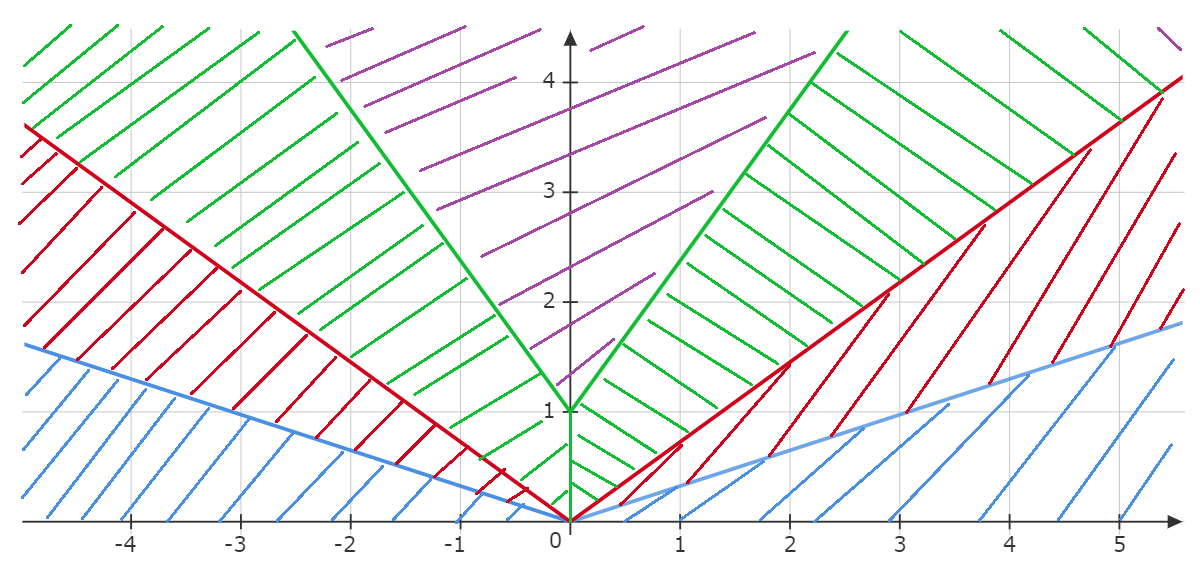
\includegraphics[width=0.5\textwidth]{AlphaFirstDecomposition.png}
	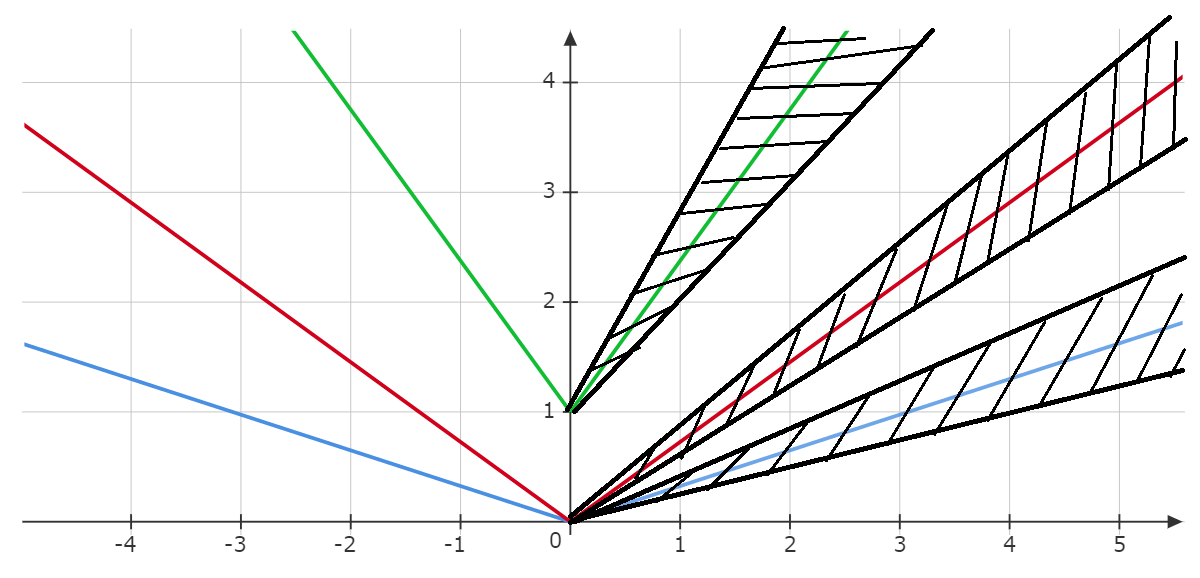
\includegraphics[width=0.5\textwidth]{AlphaSecondDecomposition.png}
	\caption{This figure shows the support of the different automorphisms present in the decomposition of an SQ-automorphism acting on the upper half plane.}
\end{figure}
 As a remark, notice that this definition is not exactly identical to de definition given in \cite{ogata2021h3gmathbb} due to the translation operators.
 \begin{definition}
 	Take $\alpha\in\Aut{\AA}$. We say that $\alpha\in\textrm{HAut}(\AA)$ if and only if for any $0<\theta<\pi/2$ there exists an $a\in\AA$ and some $\alpha_\sigma\in\Aut{\AA_{C_\theta}\cap\AA_\sigma}$ for each $\sigma\in\{L,R\}$ such that
 	\begin{equation}
 		\alpha=\Ad{a}\circ\alpha_L\otimes\alpha_R.
 	\end{equation}
 \end{definition}
We will need one additional class of automorphisms:
\begin{definition}
	Take $\alpha\in\Aut{\AA}$. We say that $\alpha\in\textrm{VAut}(\AA)$ if and only if there exists some $a\in\AA$, $\alpha_U\in\Aut{\tau(\AA_{C_\theta^c}\cap\AA_{U})}$ and an $\alpha_D\in\Aut{\tau^{-1}(\AA_{C_\theta^c}\cap\AA_{D})}$ such that
	\begin{equation}
		\alpha=\Ad{a}\circ\alpha_U\otimes\alpha_D.
	\end{equation}
	If furthermore $\alpha_U\circ\beta_g^U=\beta_g^U\circ\alpha_U$ we say that $\alpha\in\textrm{GVAut}(\AA)$.
\end{definition}
Now we will state some properties of locally generated automorphisms:
\begin{lemma}\label{lem:PropertiesLocallyGeneratedAutomorphisms}
	Take $H$ an interaction such that there exists a $0<\phi<1$ satisfying that $\norm{H}_{f_\phi}\leq 1$. The following statements now hold (for any $s,t\in\RR$):
	\begin{enumerate}
		\item $\gamma^H_{s;t}\circ\gamma^{H_D}_{t;s}\otimes\gamma^{H_U}_{t;s}\in\textrm{HAut}(\AA)$.
		\item $\gamma^H_{s;t}\circ\gamma^{H_L}_{t;s}\otimes\gamma^{H_R}_{t;s}\in\textrm{VAut}(\AA)$. If additionally $H$ is a $G$-invariant interaction we even have $\gamma^{H_U}_{s;t}\otimes\gamma^{H_D}_{s;t}\in\textrm{GVQAut}(\AA)$.
		\item $\gamma^{H_U}_{s;t}\otimes\gamma^{H_D}_{s;t}\in\textrm{SQAut}(\AA)$. If additionally $H$ is a $G$-invariant interaction we even have $\gamma^{H_U}_{s;t}\otimes\gamma^{H_D}_{s;t}\in\textrm{GSQAut}(\AA)$.
		\item $\gamma^{H}_{t;s}\circ\beta_g^U\circ\gamma^{H}_{s;t}\circ(\beta_g^U)^{-1}\in\textrm{HAut}(\AA)$.
		\item $\gamma^{H}_{t;s}\in\textrm{SQAut}(\AA)$.
	\end{enumerate}
\end{lemma}
\begin{proof}
	Part 1 is done in Proposition 5.5 in \cite{ogata2021h3gmathbb} and part 4 follows trivially from Part 1. Except for the translation operators in my definition of the $\textrm{SQAut}(\AA)$, part 3 follows from Theorem 5.2 in \cite{ogata2021h3gmathbb}. To show part 3 we therefore have to show that Theorem 5.2 in \cite{ogata2021h3gmathbb} still holds if we replace $\mathcal{C}_0$ and $\mathcal{C}_1$ in the proof by
	\begin{align}
		\mathcal{C}_0&\defeq \left\{C_{[0,\theta_1],\sigma},C_{]\theta_1,\theta_2],\sigma,\rho},C_{]\theta_2,\theta_3],\sigma,\rho}\cup\tau^{\rho}(C_{]\theta_2,\theta_3],\sigma,\rho}),\tau^\rho(C_{]\theta_3,\pi/2],\rho})|\sigma=\{L,R\},\rho=\{U,D\}\right\}\\
		\mathcal{C}_1&\defeq\{C_{[\theta_{0.8},\theta_{1.2}]\cap\sigma\cap\tau},C_{[\theta_{1.8},\theta_{2.2}]\cap\sigma\cap\tau},\tau^\rho(C_{[\theta_{2.8},\theta_{3.2}]\cap\sigma\cap\rho})|\sigma=\{L,R\},\rho=\{U,D\}\}.
	\end{align}
	Take the $\Psi$ from this proof to be our $H$, take $\Psi^{(0)}$ to be $\sum_{C\in\mathcal{C}_0}H_{C}$ (with our new definition of $\mathcal{C}_0$) and take $\Psi^{(1)}\defeq \Psi-\Psi^{(0)}$. Now define $\Xi^{(s)}(Z,t)$ through
	\begin{equation}\label{eq:PropertiesLocallyGeneratedAutomorphismsProofDefinitionXi}
		\Xi^{(s)}(Z,t)\defeq\sum_{m=0}^\infty \sum_{\substack{X\subset Z,\\X(m)=Z}}\Delta_{X(m)}(\gamma^\Psi_{s;t}(\Psi^{(1)}(X;t)))
	\end{equation}
	with these new definitions of $\Psi^{(0)}$ and $\Psi^{(1)}$. We now want so show that for every $t$,
	\begin{equation}
		\sum_{Z\subset\ZZ^2}\left(\Xi^{(s)}(Z,t)-\sum_{C\in\mathcal{C}_1}\id_{Z\subset C}\Xi^{(s)}(Z,t)\right)
	\end{equation}
	is bounded. Following the arguments in equation (5.22) to (5.24) in \cite{ogata2021h3gmathbb} we still get that
	\begin{equation}
		\sum_{\substack{Z\subset\ZZ^2,\\\nexists C\in\mathcal{C}_1:Z\subset C}}\sup_{t\in[0,1]}\norm{\Xi^{(1)}(Z,t)}\leq \frac{8}{C_F}(e^{2I_F(\Psi)}-1)\sum_{\substack{C_1,C_2\in\mathcal{C}_0,\\ C_1\neq C_2}}M(C_1,C_2)
	\end{equation}
	where
	\begin{equation}
		M(C_1,C_2)\defeq \sum_{m\geq 0}\sum_{\substack{X:\\\forall C\in\mathcal{C}_1,X\cap((C^c)(m))\neq\emptyset,\\X\cap C_1\neq\emptyset,X\cap C_2\neq\emptyset}}\left(\sup_{t\in[0,1]}(\norm{\Psi^{(1)}(X;t)})\abs{X}G_F(m)\right)
	\end{equation}
	is now defined using the new $\mathcal{C}_1$. To bound these $M(C_1,C_2)$ we will (just like in \cite{ogata2021h3gmathbb}) differentiate between two cases. That is, the case where $C_1$ and $C_2$ are adjacent\footnote{We say that $C_1$ and $C_2$ are adjacent if and only if $\#(C_1(1)\cap C_2(1))=\infty$.} and the case where they are not. We begin with the latter. In this case we still have in complete analogy with the proof in \cite{ogata2021h3gmathbb} that
	\begin{align}
		M(C_1,C_2)\leq b_0(C_1,C_2) &\defeq \sum_{m\geq 0}\sum_{\substack{X:X\cap C_1\neq\emptyset,\\X\cap C_2\neq\emptyset}}\left(\sup_{t\in[0,1]}(\norm{\Psi^{(1)}(X;t)})\abs{X}G_F(m)\right)\\
		&\leq \norm{\Psi_1}_F\sum_{\substack{x\in C_1\\y\in C_2}}F(d(x,y))\sum_{m=0}^\infty G_F(m)<\infty.
	\end{align}
	What is now left to show is the case where $C_1$ and $C_2$ are adjacent. Take $\tilde{C}\in\mathcal{C}_1$ such that $C_1\cap\tilde{C}\neq\emptyset$ and $C_2\cap\tilde{C}\neq\emptyset$. Take $L_1=\partial\tilde{C}/C_2$\footnote{Here $\partial \tilde{C}$ means the boundary of $\tilde C$.} and $L_2=\partial\tilde{C}/C_1$. By following the same reasoning that led to equation (5.36) in \cite{ogata2021h3gmathbb} we get that
	\begin{align}
		M(C_1,C_2)\leq b_0(C_1,C_2/\tilde{C})+b_0(C_1/\tilde{C},C_2)+b_0(\tilde{C}\cap C_2,(C_1\cup C_2)^c)+b_1(C_1\cap\tilde{C},C_2\cap\tilde{C},L_1,L_2)
	\end{align}
	where
	\begin{align}
		b_1(C_1\cap\tilde{C},C_2\cap\tilde{C},L_1,L_2)&\defeq\sum_{m=0}^\infty \sum_{\substack{X\subset \tilde{C}:\\ X\cap C_1\cap\tilde{C}\neq\emptyset\\X\cap C_2\cap\tilde{C}\neq\emptyset\\ X\cap (\tilde{C}^c(m))\neq\emptyset}}\sup_{t\in[0,1]}\norm{\Psi(X;t)}\abs{X}G_F(m)\\
		&\leq \norm{\Psi_1}_F\sum_{m=0}^{\infty}G_F(m)\left(\sum_{\substack{x\in C_2\cap\tilde{C},\\y\in L_1(m)}}+\sum_{\substack{x\in C_1\cap\tilde{C},\\y\in L_2(m)}}\right)F(d(x,y))<\infty.
	\end{align}
	\footnote{Here $\Psi_1$ is defined through $\Psi_1(X)=\abs{X}^1 \Psi(X)$.} Since the remainder of the proof can remain unchanged from \cite{ogata2021h3gmathbb}, this concludes the proof of item 3. The proof of item 5 just follows from the fact that for any $\alpha_1\in\textrm{SQAut}(\AA)$ and for any $\alpha_2\in\textrm{HAut}(\AA)$ we have that $\alpha_2\circ\alpha_1\in\textrm{SQAut}(\AA)$. We now only need to comment on item 2. We must show that
	\begin{equation}
		(\gamma^H_{s;t}\circ\gamma^{H_L}_{t;s}\otimes\gamma^{H_R}_{t;s})^{-1}=\gamma^{H_L}_{s;t}\otimes\gamma^{H_R}_{s;t}\circ\gamma^H_{t;s}\in\textrm{GVAut}(\AA).
	\end{equation}
	The proof of this starts analogously to the proof of item 1 and 3. We take $\Psi=H$, $\Psi^{(0)}=H_{\tau(C_\theta^c\cap U)}+H_{\tau^{-1}(C_\theta^c\cap D)}$ and $\Psi^{(1)}=\Psi-\Psi^{(0)}$. Define $\Xi^{(s)}(Z;t)$ again through equation \eqref{eq:PropertiesLocallyGeneratedAutomorphismsProofDefinitionXi}. In analogy to what was done in equation (5.54) in \cite{ogata2021h3gmathbb} we obtain
	\begin{equation}
		\sum_{\substack{Z:Z\nsubseteq \tau(C_\theta^c\cap U)\\\text{and }Z\nsubseteq \tau^{-1}(C_\theta^c\cap D)}}\sup_{t\in[0,1]}\norm{\Xi^{(1)}(Z,t)}\leq \frac{8}{C_F}(e^{2I_F(\Psi)}-1)\sum_{m=0}^\infty\sum_{\substack{Z:Z(m)\nsubseteq \tau(C_\theta^c\cap U)\\\text{and }Z(m)\nsubseteq \tau^{-1}(C_\theta^c\cap D)}} \sup_{t\in[0,1]}\norm{\Psi^{(1)}(X;t)}\abs{X}G_F(m).
	\end{equation}
	If $X$ in the last line has a non-zero contribution, then at least one of the following occurs:
	\begin{enumerate}
		\item $X\cap (W(C_\theta)\cap L)\neq\emptyset$ and $X\cap R\neq\emptyset$.
		\item $X\cap (W(C_\theta)\cap R)\neq\emptyset$ and $X\cap L\neq\emptyset$.
		\item $X\subset W(C_\theta)^c$ and
		\begin{enumerate}
			\item $X\subset U,X\subset D$, or
			\item $X\subset U,X\subset L,X\subset R$ and $X(m)\cap (\tau^{-1}(C_\theta^c\cap D))^c\neq \emptyset$, or
			\item $X\subset D,X\subset L,X\subset R$ and $X(m)\cap (\tau(C_\theta^c\cap U))^c\neq \emptyset$.
		\end{enumerate}
	\end{enumerate}
	This shows that we have a bound
	\begin{align}
		&\sum_{\substack{Z:Z\nsubseteq \tau(C_\theta^c\cap U)\\\text{and }Z\nsubseteq \tau^{-1}(C_\theta^c\cap D)}}\sup_{t\in[0,1]}\norm{\Xi^{(1)}(Z,t)}\\
		\nonumber
		&\leq \frac{8}{C_F}(e^{2I_F(\Psi)}-1)(b_0(W(C_\theta)\cap L,R)+b_0(L,W(C_\theta)\cap R)+b_0(W(C_\theta)^c\cap U,W(C_\theta)^c\cap D)\\
		\nonumber
		&\qquad+b_1(W(C_\theta)^c\cap U\cap L,W(C_\theta)^c\cap U\cap L,L\cap\partial(W(C_\theta)^c\cap U),R\cap\partial(W(C_\theta)^c\cap U))\\
		&\qquad b_1(W(C_\theta)^c\cap D\cap L,W(C_\theta)^c\cap D\cap R,L\cap\partial(W(C_\theta)^c\cap D),R\cap\partial(W(C_\theta)^c\cap D)))<\infty.
	\end{align}
	This concludes the proof.
\end{proof}
This implies certain things for our locally generated automorphisms.
From these four statements we can prove the following results:
\begin{lemma}\label{lem:TwoAngleLemmaPart1}
	Take $\theta_1$ and $\theta_2$ such that $0<\theta_1<\theta_2<\pi/2$ then for all $\Theta\in\Aut{\AA_{W(C_{\theta_2})^c}}$ and $s,t\in\RR$ there exists an $a_1\in\UU(\AA)$ and a $\tilde{\Theta}\in \Aut{\AA_{W(C_{\theta_1})^c}}$ such that
		\begin{equation}\label{eq:TwoAngleLemmaPart1Equation1}
			\gamma^{H}_{t;s}\circ\Theta\circ\gamma^{H}_{s;t}=\Ad{a_1}\circ\tilde{\Theta}.
		\end{equation}
\end{lemma}
\begin{proof}
	We have that
	\begin{equation}
		\gamma^{H}_{t;s}\circ\Theta\circ\gamma^{H}_{s;t}=\gamma^{H_D}_{t;s}\otimes\gamma^{H_U}_{t;s}\circ\gamma^{H_D}_{s;t}\otimes\gamma^{H_U}_{s;t}\circ\gamma^{H}_{t;s}\circ\Theta\circ\gamma^{H}_{s;t}\circ\gamma^{H_D}_{t;s}\otimes\gamma^{H_U}_{t;s}\circ\gamma^{H_D}_{s;t}\otimes\gamma^{H_U}_{s;t}.
	\end{equation}
	Using that $\gamma^{H}_{s;t}\circ\gamma^{H_D}_{t;s}\otimes\gamma^{H_U}_{t;s}\in\textrm{HAut}(\AA)$ we get that there exists some $a\in\AA$ and $\eta\in\Aut{\AA_{C_\theta}}$ such that
	\begin{align}
		\gamma^{H}_{t;s}\circ\Theta\circ\gamma^{H}_{s;t}&=\Ad{a}\circ \gamma^{H_D}_{t;s}\otimes\gamma^{H_U}_{t;s}\circ\eta_{s;t}^{-1}\circ\Theta\circ\eta_{s;t}\circ\gamma^{H_D}_{s;t}\otimes\gamma^{H_U}_{s;t}\\
		&=\Ad{a}\circ \gamma^{H_D}_{t;s}\otimes\gamma^{H_U}_{t;s}\circ\Theta\circ\gamma^{H_D}_{s;t}\otimes\gamma^{H_U}_{s;t}.
	\end{align}
	Since by \ref{lem:PropertiesLocallyGeneratedAutomorphisms} part 3 $\gamma^{H_D}_{s;t}\otimes\gamma^{H_U}_{s;t}\in\textrm{GSQAut}(\AA)$ the result follows. {\color{red}Do I have to explain this further?}
\end{proof}
\begin{lemma}\label{lem:TwoAngleLemmaPart2}
	Take $\theta_1$ and $\theta_2$ such that $0<\theta_1<\theta_2<\pi/2$. Then for all $\eta_{g}^{\sigma}\in\Aut{\AA_{C_{\theta_1}}\cap\AA_{\sigma}}$ (where $\sigma\in\{L,R\}$ and $g\in G$) and $s,t\in\RR$ there exist $a_{2},\in\UU(\AA),a_{3,\sigma}\in\UU(\AA_\sigma)$ and some $\tilde{\eta}_{\sigma}^g\in \Aut{\AA_{C_{\theta_2}}\cap\AA_{\sigma}}$ such that
	\begin{align}
		\label{eq:TwoAngleLemmaPart2Equation1}
		\gamma^{H}_{t;s}\circ\eta_{g}^L\otimes\eta_{g}^R\circ\gamma^{H}_{s;t}&=\Ad{a_2}\circ(\tilde\eta_{g}^L \otimes\tilde\eta_{g}^R)\\
		\label{eq:TwoAngleLemmaPart2Equation2}
		\gamma^{H_\sigma}_{t;s}\eta_g^\sigma\gamma^{H_\sigma}_{s;t}&=\Ad{a_{3,\sigma}}\circ \tilde\eta_{g}^\sigma.
	\end{align}
\end{lemma}
\begin{proof}
	First we show that equation \eqref{eq:TwoAngleLemmaPart2Equation2} implies equation \eqref{eq:TwoAngleLemmaPart2Equation1}. This is because using equation \eqref{eq:TwoAngleLemmaPart2Equation1} we get that
	\begin{align}
		\gamma^H_{t;s}\circ\eta_g\circ\gamma^{H}_{s;t}&=\gamma^H_{t;s}\circ\gamma^{H_L}_{s;t}\otimes\gamma^{H_R}_{s;t}\circ\gamma^{H_L}_{t;s}\otimes\gamma^{H_R}_{t;s}\circ\eta_g\circ\gamma^{H_L}_{s;t}\otimes\gamma^{H_R}_{s;t}\circ\gamma^{H_L}_{t;s}\otimes\gamma^{H_R}_{t;s}\circ\gamma^H_{s;t}\\
		&=\gamma^H_{t;s}\circ\gamma^{H_L}_{s;t}\otimes\gamma^{H_R}_{s;t}\circ\Ad{a_{3,L}\otimes a_{3,R}}\circ\tilde{\eta}_g\circ\gamma^{H_L}_{t;s}\otimes\gamma^{H_R}_{t;s}\circ\gamma^H_{s;t}.
	\end{align}
	If one now uses the fact that $\gamma^H_{t;s}\circ\gamma^{H_L}_{s;t}\otimes\gamma^{H_R}_{s;t}\in\textrm{GVAut}(\AA)$ the implication follows.
\end{proof}
\bibliography{TSPT}
\bibliographystyle{plain}
\end{document}